\chapter{Umsetzung und Evaluation des optimierten Prozesses}

\section{Lösung 1: Anpassung des Standards} \label{sec:Kapitel41}

\subsubsection{Grundlegendes}

Im Folgenden soll die Umsetzung des Soll-Konzepts durch eine Anpassung des SAP-Standards vorgestellt werden. Des geschieht konkret durch ein Customizing der Fiori-App ''Massenänderungen an zentralen Einkaufskontrakten''. SAP Fiori ist ein Framework für die Entwicklung und Bereitstellung von SAP-Apps. Durch ein einheitliches und rollenbasiertes Layout entsteht eine intuitiv bedienbare und konsistente Benutzeroberfläche. Da Fiori Apps responsive sind, können diese auf verschiedenen Endgeräten genutzt werden, um die Produktivität der Nutzer zu steigern. Insgesamt soll Fiori die UX von SAP-Anwendungen, vor allem für unerfahrenere Nutzer, verbessern.\footcite[Vgl.][]{praxis_sap_fiori_allgemein_2024}

\subsubsection{Aufbau der App}

\begin{figure}[H]
    \centering
    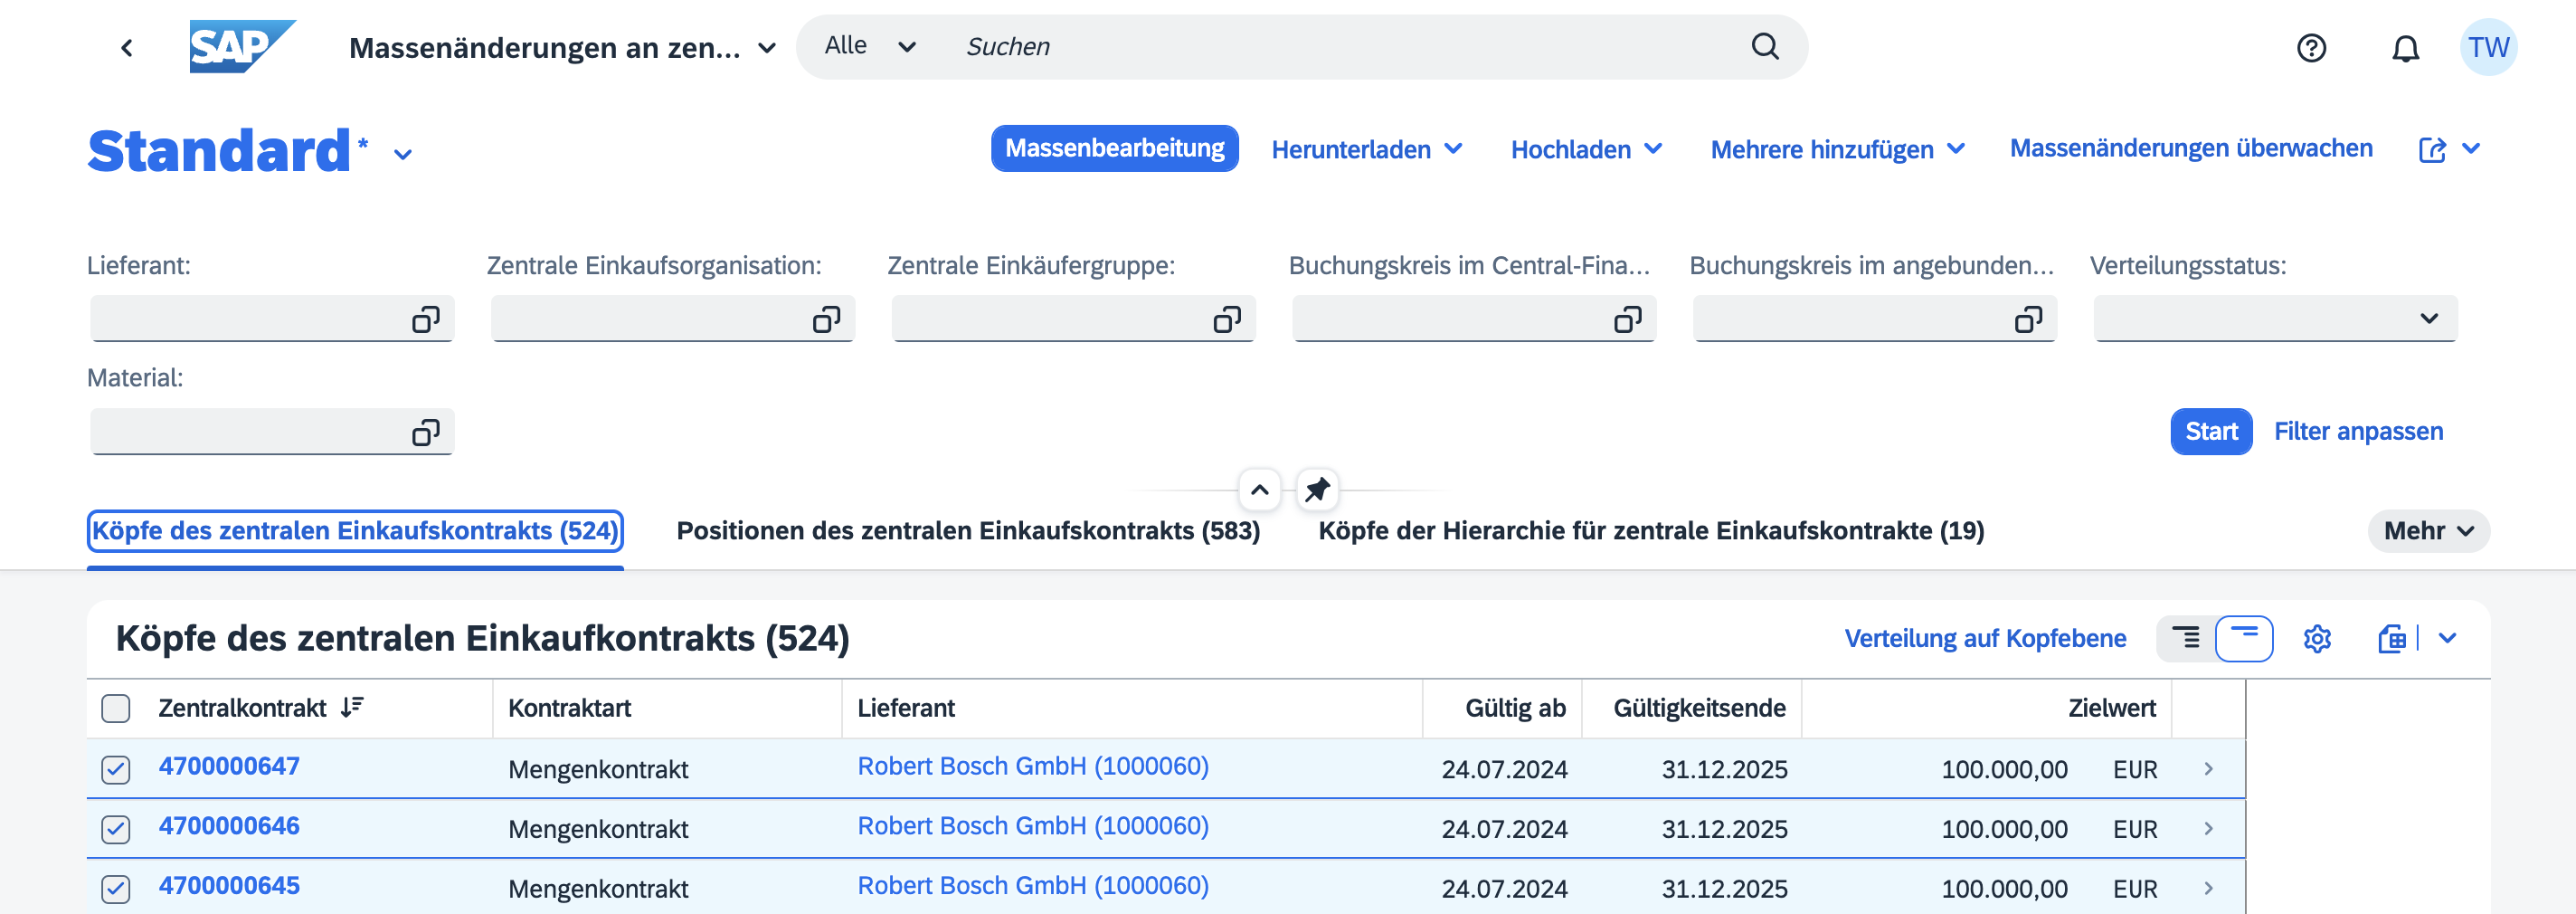
\includegraphics[height=5.31cm]{Bilder/Praxisteil-S-Schritt-1.png}
    \caption[Standard Customizing, Massenbearbeitung Central Contracts, Auswahl der Zentralkontrakte]{Standard Customizing, Massenbearbeitung Central Contracts, Auswahl der Zentralkontrakte. Eigene Darstellung}
    \label{fig:PraxisSSchritt1}
\end{figure}

Zuerst wird der allgemeine Prozessfluss und Aufbau der App beschrieben. Einschränkend ist zu nennen, dass die Fiori-App selbst, aufgrund von Einschränkungen der Software durch SAP, nicht anpassbar ist. Deshalb müssen die folgenden Ausführungen als gegeben angenommen werden. Dies hat zur Folge, dass das Konzept im Bezug auf die Prozessstruktur nicht exakt umgesetzt werden kann. Abbildung \ref{fig:PraxisSSchritt1} zeigt den Einstiegspunkt eines Benutzers nach dem Öffnen der App. Im oberen Bereich der Seite befindet sich die allgemeine Fiori Navigation, über die die App-Übersichtsseite oder -Suche erreicht werden kann. Zudem befinden sich rechts oben das Benutzerprofil und Benachrichtigungen. Darunter können die Ansicht der App ausgewählt und verschiedene Aktionen ausgeführt werden. Der Button ''Massenbearbeitung'' führt den Online-Massenänderungsmodus aus. Dieser bietet die Möglichkeit ein oder mehrere Felder in allen ausgewählten Verträgen mit einem Wert zu überschreiben. Da dies nicht das Ziel des Konzepts ist, wird diese Funktion im Folgenden au\ss er Acht gelassen. Konkret wird die Offline-Massenänderung betrachtet: Hier können über die Knöpfe ''Herunterladen'' und ''Hochladen'' eine Excel-Datei herunter- und wieder hochgeladen werden. Nachdem die Datei mit den jeweiligen Ist-Daten heruntergeladen wurde, können innerhalb der Systemgrenzen beliebige Änderungen vorgenommen werden. Beispielsweise können für verschiedene Verträge/ Vertragspositionen jeweils anders geändert werden. Zudem können auch komplette Zentralkontrakte hinzugefügt oder gelöscht werden. Nachdem alle Änderungen vorgenommen wurden, wird die Excel-Liste wieder ins System hochgeladen. An diesem Punkt kann sich der Einkäufer entscheiden, ob die Änderungen direkt übernommen, oder zuerst eine Simulation durchgeführt werden soll.\footcite[Vgl.][]{theorie_sap_fiori_make_mass_changes_2024} Über den Button ''Massenänderungen überwachen'' öffnet sich die gleichnamige App und der Benutzer kann in beiden Fällen das Ergebnis mit eventuellen Warnungen und Fehlermeldungen einsehen. Im Falle der Simulation kann diese hier final im System übernommen oder verworfen werden.\footcite[Vgl.][]{theorie_sap_fiori_monitor_mass_changes_2024} Die Funktion ''Weitere hinzufügen'' ermöglicht es, Verteilungsschlüssel festzulegen, die bestimmen, welche Mengen welcher Teile in den gewählten Verträgen für welche Werke bestimmt sind. Letztere ist ebenfalls im Anwendungskontext nicht relevant. Unter den eben genannten Knöpfen befinden sich Filtermöglichkeiten, um die Anzeige der Verträge zu verfeinern. Im Auswahlbereich der App stehen dem Facheinkäufer drei Bereiche zur Verfügung: Köpfe und Positionen zentraler Einkaufskontrakte, sowie dieselben Möglichkeiten der Hierarchie der zentralen Einkaufskontrakte. Da die letztere Möglichkeit von BMW nicht eingesetzt wird, wird diese nachfolgend nicht betrachtet. Allgemein lässt sich sagen, dass Massenänderungen auf Vertragsebene oder auf Positionsebene vorgenommen werden können. Der Endanwender kann nun die gewünschten Verträge, sowie zugehörigen Positionen, die er bearbeiten möchte selektieren. Im Kundenkontext ist dies trivial, da jeder Vertrag nur eine Position enthält. Diese werden in einer Tabelle aufgelistet. In Abbildung \ref{fig:PraxisSSchritt1} werden in den Spalten noch die Attribute des Standards angezeigt, diese können jedoch analog zu den in \ref{sec:Kapitel422} gewählten Attributen angepasst werden.

\subsubsection{Massenbearbeitung in Excel}

Nachdem der Einkäufer die gewünschten Zentralkontrakte inklusive Positionen selektiert hat, können deren Daten als Excel Datei angepasst werden. In diesem Bereich ist die SAP-Lösung flexibel konfigurierbar. So können benutzerdefiniert mehrere Arbeitsblätter angelegt und diese fast beliebig mit Feldern des Central Contracts befüllt werden. Im Folgenden soll diese Excel-Datei vorgestellt werden. Jede zu bearbeitende Kategorie wird durch ein Tabellenblatt dargestellt. Der Umfang der Massenbearbeitung kann leider nicht angepasst werden, da, wie oben dargestellt, die Fiori-App nicht verändert werden kann. Daraus resultiert, dass \zB einzelne Kategorien, die in einem bestimmten Fall garnicht bearbeitet würden, trotzdem in der Excel-Datei vorhanden sind. Auch innerhalb der Kategorien können keine bestimmten Konditionen/ Rohstoffe, die zusätzlich zu den bestehenden angezeigt werden sollen, selektiert werden. Diese müssen manuell vom Facheinkäufer hinzugefügt werden. 

\begin{figure}[H]
    \centering
    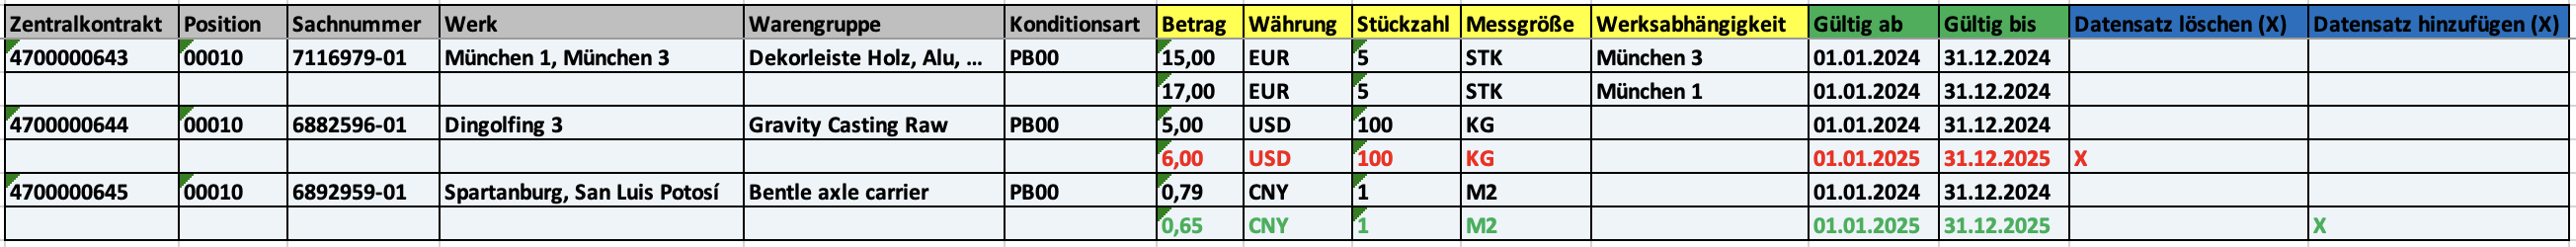
\includegraphics[height=1.43cm]{Bilder/Praxisteil-S-Schritt-2.png}
    \caption[Standard Customizing, Massenbearbeitung Central Contracts, Bearbeitung des Basispreises]{Standard Customizing, Massenbearbeitung Central Contracts, Bearbeitung des Basispreises. Eigene Darstellung}
    \label{fig:PraxisSSchritt2}
\end{figure}

Abbildung \ref{fig:PraxisSSchritt2} stellt die Bearbeitung des Basispreises im ersten Schritt dar. Allgemein sind Spalten, deren Spaltenköpfe grau markiert sind lediglich informativ, um dem Einkäufer die Identifikation der gewählten Verträge zu erleichtern. Letztere werden sich in allen Kategorien bis auf der zu bearbeitenden Kondition gleichen. Spalten mit gelben Spaltenköpfen enthalten fachliche Daten des Zentralkontrakts, die editiert werden dürfen. Die PME wurde in die Felder Stückzahl und Messgrö\ss e aufgeteilt, um die Dateneingabe und -verarbeitung zu erleichtern. Grün hinterlegte Spaltenköpfe enthalten die zeitlichen Gültigkeiten einzelner Konditionen/ Rohstoffe. Aus Übersichtlichkeitsgründen wurden hier nur zwei Zeitintervalle dargestellt. Diese können aufgrund von Limitationen der Software nicht in einen Vorauswahlschritt extrahiert werden. Die blauen Spalten sind lediglich technischer Natur, falls ein Facheinkäufer einen Datensatz hinzufügen oder löschen möchte. In diesem Fall müsste eine der beiden Spalten mit ''X'' markiert werden. Sollte ein Datensatz so gelöscht werden, wird jedoch nur \zB die jeweilige Kondition/ Rohstoff gelöscht, nicht die gesamte Vertragsposition oder der gesamte Vertrag. Beispielsweise wird in Abbildung \ref{fig:PraxisSSchritt2} in der vierten Zeile ein Basispreisintervall gelöscht. Wenn beispielsweise eine neue Kondition hinzugefügt werden soll, muss eine neue Spalte eingefügt, die jeweiligen Daten eingegeben und die Spalte ''Datensatz hinzufügen'' markiert werden, wie in der letzten Zeile von Abbildung \ref{fig:PraxisSSchritt2} in grüner Schrift zu sehen. Da die Massenbearbeitung nicht auf ein Zeitintervall eingegrenzt werden kann, werden pro Vertrag alle Basispreiszeiträume untereinander aufgelistet und der Endanwender muss für jede Änderung ein gegebenenfalls anderes Zeitintervall pflegen. Sollten werksabhängige Basispreise pro Zeitraum existieren, werden diese ebenfalls untereinander aufgelistet. Aufgrund der Systemfunktionalität wird der Basispreis, sowie Konditionen und Rohstoffe nur mittels der technischen Abkürzungen dargestellt, welche dem Facheinkäufer bekannt sein müssen. Dieses Schema wird für alle folgenden Kategorien analog übernommen.

\begin{figure}[H]
    \centering
    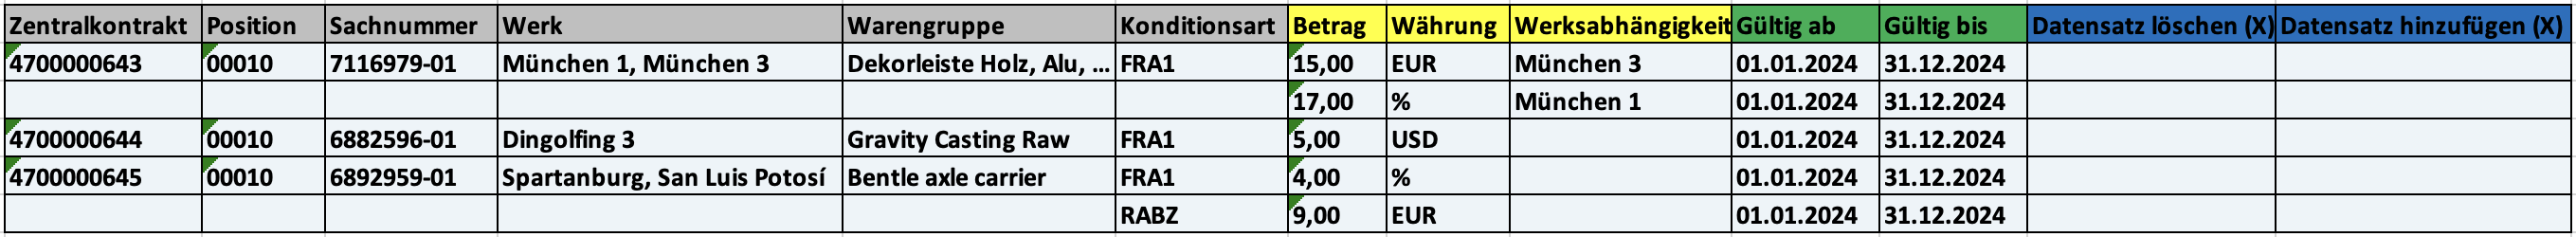
\includegraphics[height=1.38cm]{Bilder/Praxisteil-S-Schritt-3.png}
    \caption[Standard Customizing, Massenbearbeitung Central Contracts, Bearbeitung der Zu- und Abschläge]{Standard Customizing, Massenbearbeitung Central Contracts, Bearbeitung der Zu- und Abschläge. Eigene Darstellung}
    \label{fig:PraxisSSchritt3}
\end{figure}

Im nächsten Schritt können, wie in Abbildung \ref{fig:PraxisSSchritt3} dargestellt, die Zu- und Abschläge bearbeitet werden. Diese werden pro Zentralkontrakt in Zeilen untereinander aufgelistet. Im konkreten Beispiel hat der erste Vertrag einen werksabhängigen Frachtzuschlag mit unterschiedlichen Werten je Werk. Der dritte Vertrag hat zu diesem Zuschlag noch einen Verpackungszuschlag. Im Unterschied zum Basispreis existiert das Feld PME nicht, da sich diese Konditionsart immer auf den gesamten Basispreis und nicht auf eine bestimmte Mengeneinheit bezieht. Des Weiteren kann ein Zu- bzw. Abschlag auch in Prozent auf den Basispreis angegeben werden. Das Feld ''Betrag'' wird automatisch in Abhängigkeit davon, ob ein Währungscode oder ''\%'' angegeben wurde interpretiert, sodass keine Umrechnung in verschiedene Dezimalstellen notwendig ist. Beispielsweise kann der Einkäufer einen Frachtzuschlag von 0,5\% als ''0,5'' eingeben und muss diesen nicht als ''0,005'' eingeben.

\begin{figure}[H]
    \centering
    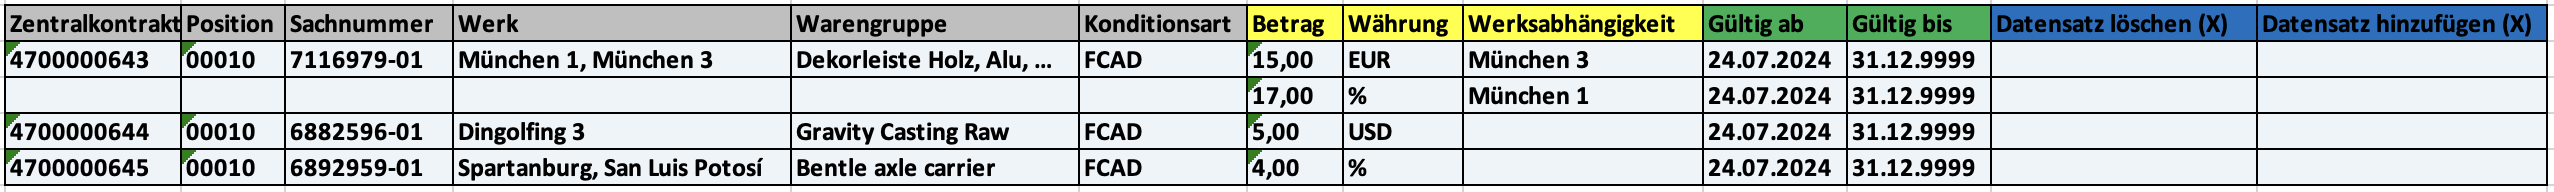
\includegraphics[height=1.12cm]{Bilder/Praxisteil-S-Schritt-4.png}
    \caption[Standard Customizing, Massenbearbeitung Central Contracts, Bearbeitung der Fremdwährungen]{Standard Customizing, Massenbearbeitung Central Contracts, Bearbeitung der Fremdwährungen. Eigene Darstellung}
    \label{fig:PraxisSSchritt4}
\end{figure}

Die in Abbildung \ref{fig:PraxisSSchritt4} abgebildeten Fremdwährungen sind im Bezug auf die relevanten Felder analog zu den Zu- und Abschlägen aufgebaut und spezielle Versionen letzterer. Eine Trennung findet aufgrund der User Experience der Nutzer statt, da in anderen IT-Systemen des Kunden diese Trennung von ''normalen'' Zu- und Abschlägen und Fremdwährungen ebenfalls stattfindet.

\begin{figure}[H]
    \centering
    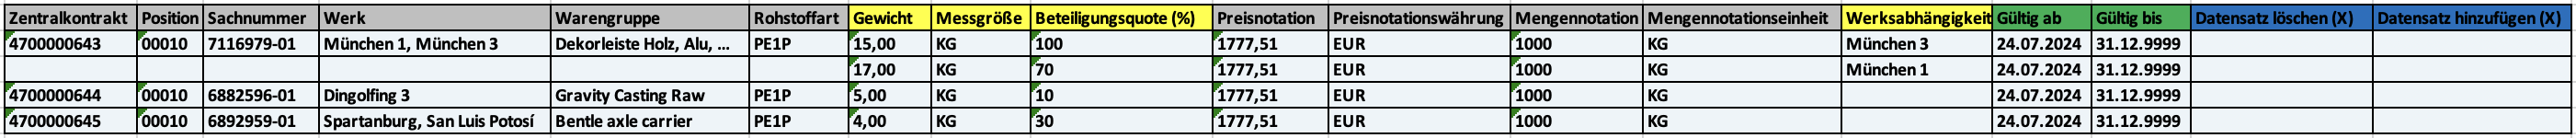
\includegraphics[height=0.8cm]{Bilder/Praxisteil-S-Schritt-5.png}
    \caption[Standard Customizing, Massenbearbeitung Central Contracts, Bearbeitung der marktorientierten Rohstoffe]{Standard Customizing, Massenbearbeitung Central Contracts, Bearbeitung der marktorientierten Rohstoffe. Eigene Darstellung}
    \label{fig:PraxisSSchritt5}
\end{figure}

Abbildung \ref{fig:PraxisSSchritt5} zeigt die Bearbeitungsmaske für marktorientierte Rohstoffe. Da deren Notation von der Börse vorgegeben wird, sind die korrespondierenden Felder in der Excel-Tabelle grau markiert und werden somit beim Upload nicht berücksichtigt. Dennoch ist die Notation in 4 Spalten aufgeteilt, um die Daten übersichtlicher darzustellen. Um die Auswirkung auf den Basispreis zu erhalten, werden Gewicht, Beteiligungsquote und die Notation des Rohstoffs multipliziert und im Hintergrund auf den Basispreis addiert. Die Beteiligungsquote gibt an, zu welchem Anteil BMW sich an dem Rohstoff-Preisbestandteil beteiligt und ist somit wichtig, um Preisschwankungen abzufedern.

\begin{figure}[H]
    \centering
    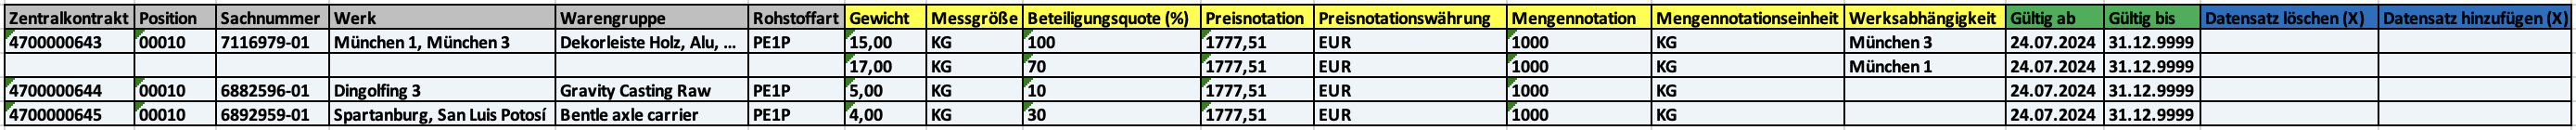
\includegraphics[height=0.75cm]{Bilder/Praxisteil-S-Schritt-6.png}
    \caption[Standard Customizing, Massenbearbeitung Central Contracts, Bearbeitung der Rohstoffe mit freier Notierung]{Standard Customizing, Massenbearbeitung Central Contracts, Bearbeitung der Rohstoffe mit freier Notierung. Eigene Darstellung}
    \label{fig:PraxisSSchritt6}
\end{figure}

Im letzten Schritt vor Upload der Excel-Datei können noch die Rohstoffe mit freier Notierung bearbeitet werden. Im Unterschied zu den RMO zeigt Abbildung \ref{fig:PraxisSSchritt6}, dass die mit der Notation zusammenhängenden Felder gelb hinterlegt, also bearbeitbar sind. Somit kann sich der Facheinkäufer mit dem Lieferanten auf einen Rohstoffpreis einigen und diesen in das System einpflegen. Die Berechnung der preislichen Auswirkungen erfolgt analog zu den RMO.

Nachdem die Bearbeitung der Excel-Liste durch den Facheinkäufer abgeschlossen ist, muss diese, wie oben dargestellt in der Fiori-App hochgeladen werden. Dies geschieht durch eine Schnittstelle zum Zentralkontrakt, über die die Daten im System geändert werden. An dieser Stelle können die Anforderungen an das Systemverhalten umgesetzt werden. Die Systemlogik kann an definierten Stellen, sogenannten ''Business Add-Ins'' (im Folgenden ''BAdI'' abgekürzt), mit kundeneigenem Programmcode erweitert oder geändert werden. Im konkreten Anwendungsfall würde der BAdI ''MM\_PUR\_S4\_CCTR\_MODIFY\_ITEM'' genutzt werden.\footcite[Vgl.][]{theorie_sap_central_contract_overview_2024} Durch letzteren ist es möglich, die Position eines Vertrags vor dem Speichern zu verändern, wodurch \zB Gültigkeitsintervalle von Basispreisen, Konditionen, oder Rohstoffen angepasst werden können. Auch kann das BMW-spezifische Prüfungsframework eingebunden und sichergestellt werden, dass die Änderungen keine Zeiträume betreffen, die je nach Benutzer, länger als zwölf bzw. 36 Monate in der Vergangenheit liegen. Nachdem die Daten ins System übertragen wurde, ist der Prozess beendet.

\section{Lösung 2: Entwicklung einer kundenspezifischen Lösung}

Die zweite Möglichkeit die Kundenanforderungen umzusetzen ist die Entwicklung einer kundenspezifischen Lösung. Allgemein bietet sich im konkreten Fall die Entwicklung einer kundeneigenen Fiori-App an, über die die Daten im System gepflegt werden können. Fiori bietet mehrere Vorlagen an, die als Basis für die Entwicklung einer App genutzt werden können. Für den betrachteten Prozess bietet sich die Vorlage ''Wizard-Floorplan'' an, da diese eine schrittweise Benutzerführung durch mehrstufige Prozesse bietet. So können komplexe Aufgaben in kleinere Schritte unterteilt werden, zwischen denen der Benutzer navigieren kann und bei denen er bei Bedarf Hilfestellungen und Fehlermeldungen erhält. So soll die UX gesteigert und die Fehlerquote gesenkt werden \parencite[Vgl.][]{praxis_sap_wizard_floorplan_2024}. Im Folgenden soll der Aufbau dieses Floorplans anhand des ersten Prozessschrittes exemplarisch beschrieben werden.

\subsubsection{Auswahl des Zeitintervalls}

\begin{figure}[H]
    \centering
    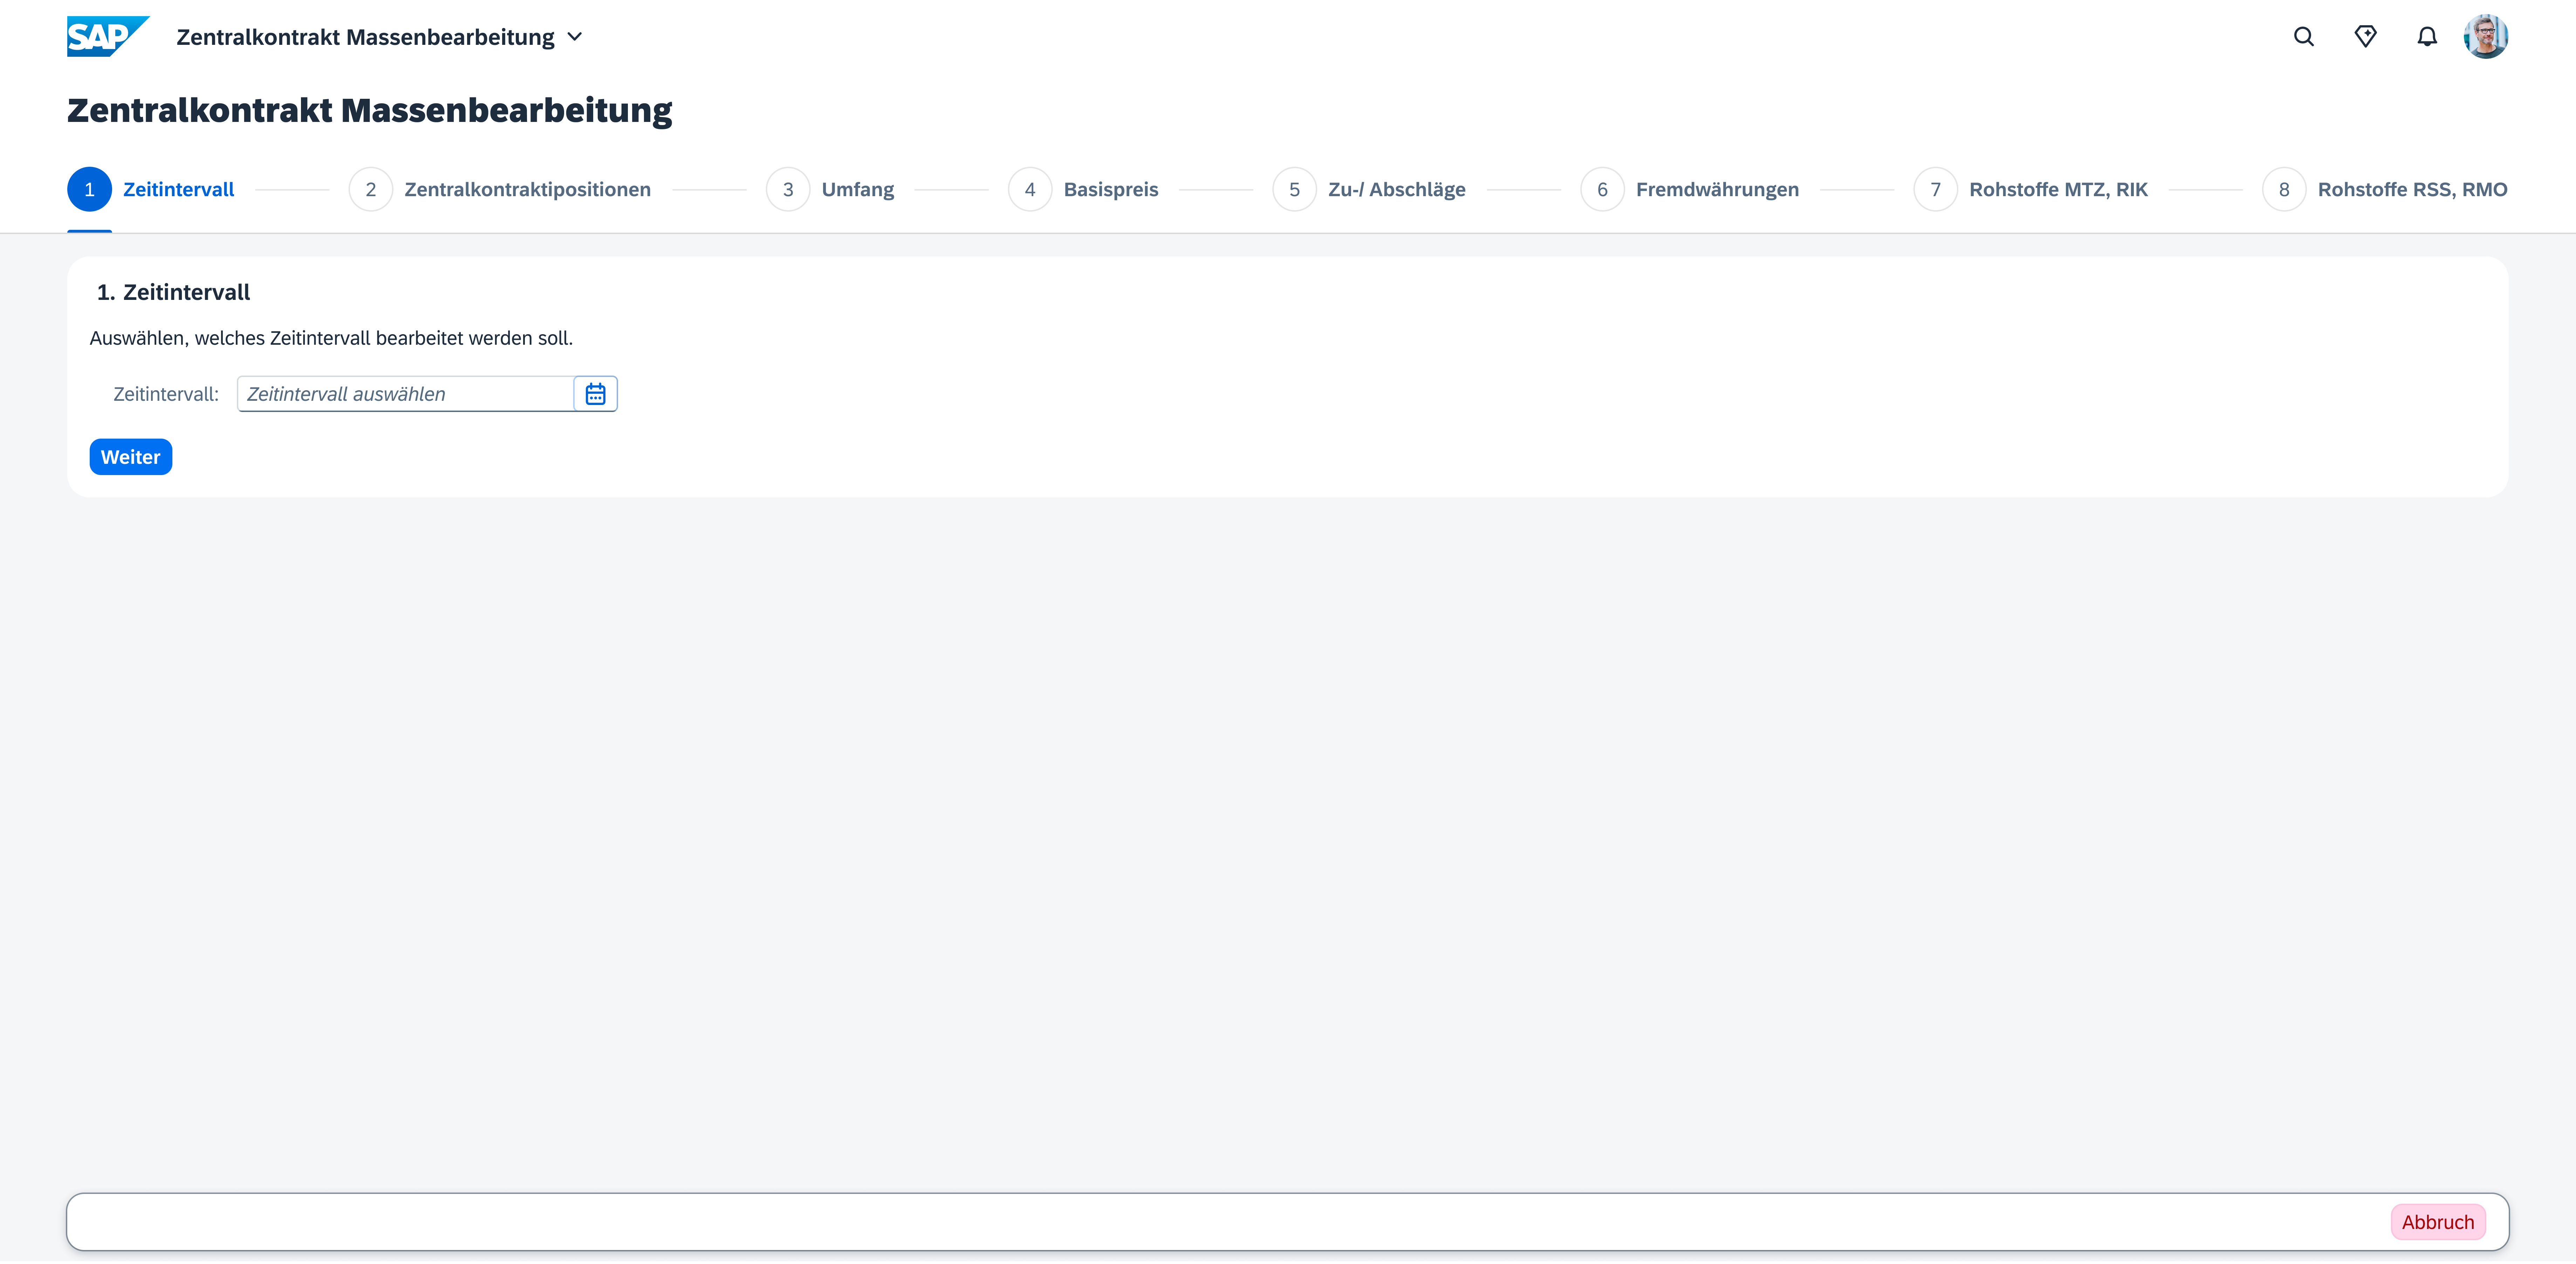
\includegraphics[height=7.37cm]{Bilder/Praxisteil-KL-Schritt-1.png}
    \caption[Kundenentwicklung, Massenbearbeitung Central Contracts, Auswahl des Zeitintervalls]{Kundenentwicklung, Massenbearbeitung Central Contracts, Auswahl des Zeitintervalls. Eigene Darstellung}
    \label{fig:PraxisKLSchritt1}
\end{figure}


In Abbildung \ref{fig:PraxisKLSchritt1} ist der erste Schritt des Prozesses dargestellt. Der Header der App enthält analog zu  Kapiel \ref{sec:Kapitel41} die allgemeine Fiori Navigation. Unter dem Titel der App befindet sich eine Übersicht über die Abfolge der Prozessschritte mit einer Anzeige über den jeweiligen Fortschritt des Prozesses. Darunter beginnt der eigentliche Inhalt der App. Dieser unterscheidet sich in jeder Phase. In der Abbildung kann der Benutzer ein Zeitintervall mithilfe eines Auswahlfeldes eingeben. In diesem Zeitintervall werden alle folgenden Änderungen vorgenommen. Sollte sich das gewählte Intervall über mehrere Instanzen des Basispreises erstrecken erscheint eine Warnung, da bei Fortfahren einzelne Intervalle nicht nur verkürzt, sondern vollständig überschrieben werden. Sollte kein oder ein ungültiges Zeitintervall ausgewählt werden, erscheint eine Fehlermeldung, und der Prozess kann nicht fortgesetzt werden, bis ein gültiger Zeitraum ausgewählt wurde. Dies gilt auch für den Fall, dass, abhängig von der jeweiligen Berechtigung eines Benutzers, ein Zeitraum von mehr als zwölf bzw. 36 Monaten in der Vergangenheit gewählt wird. Nachdem der Einkäufer einen Zeitraum durch Klicken auf den Kalender ausgewählt hat, gelangt er durch den Button ''Weiter'' zum nächsten Schritt. Alternativ kann der Benutzer den Prozess durch den Knopf ''Abbruch'' abbrechen oder durch den Button ''Zurück'' einen Schritt zurückgehen.\footnote{Der Button ist auf Abbildung \ref{fig:PraxisKLSchritt1} nicht vorhanden, da es sich um den ersten Schritt handelt. In den folgenden Schritten ist dieser in der Leiste unten links zu sehen}

\subsubsection{Auswahl der Zentralkontrakte} \label{sec:Kapitel422}

\begin{figure}[H]
    \centering
    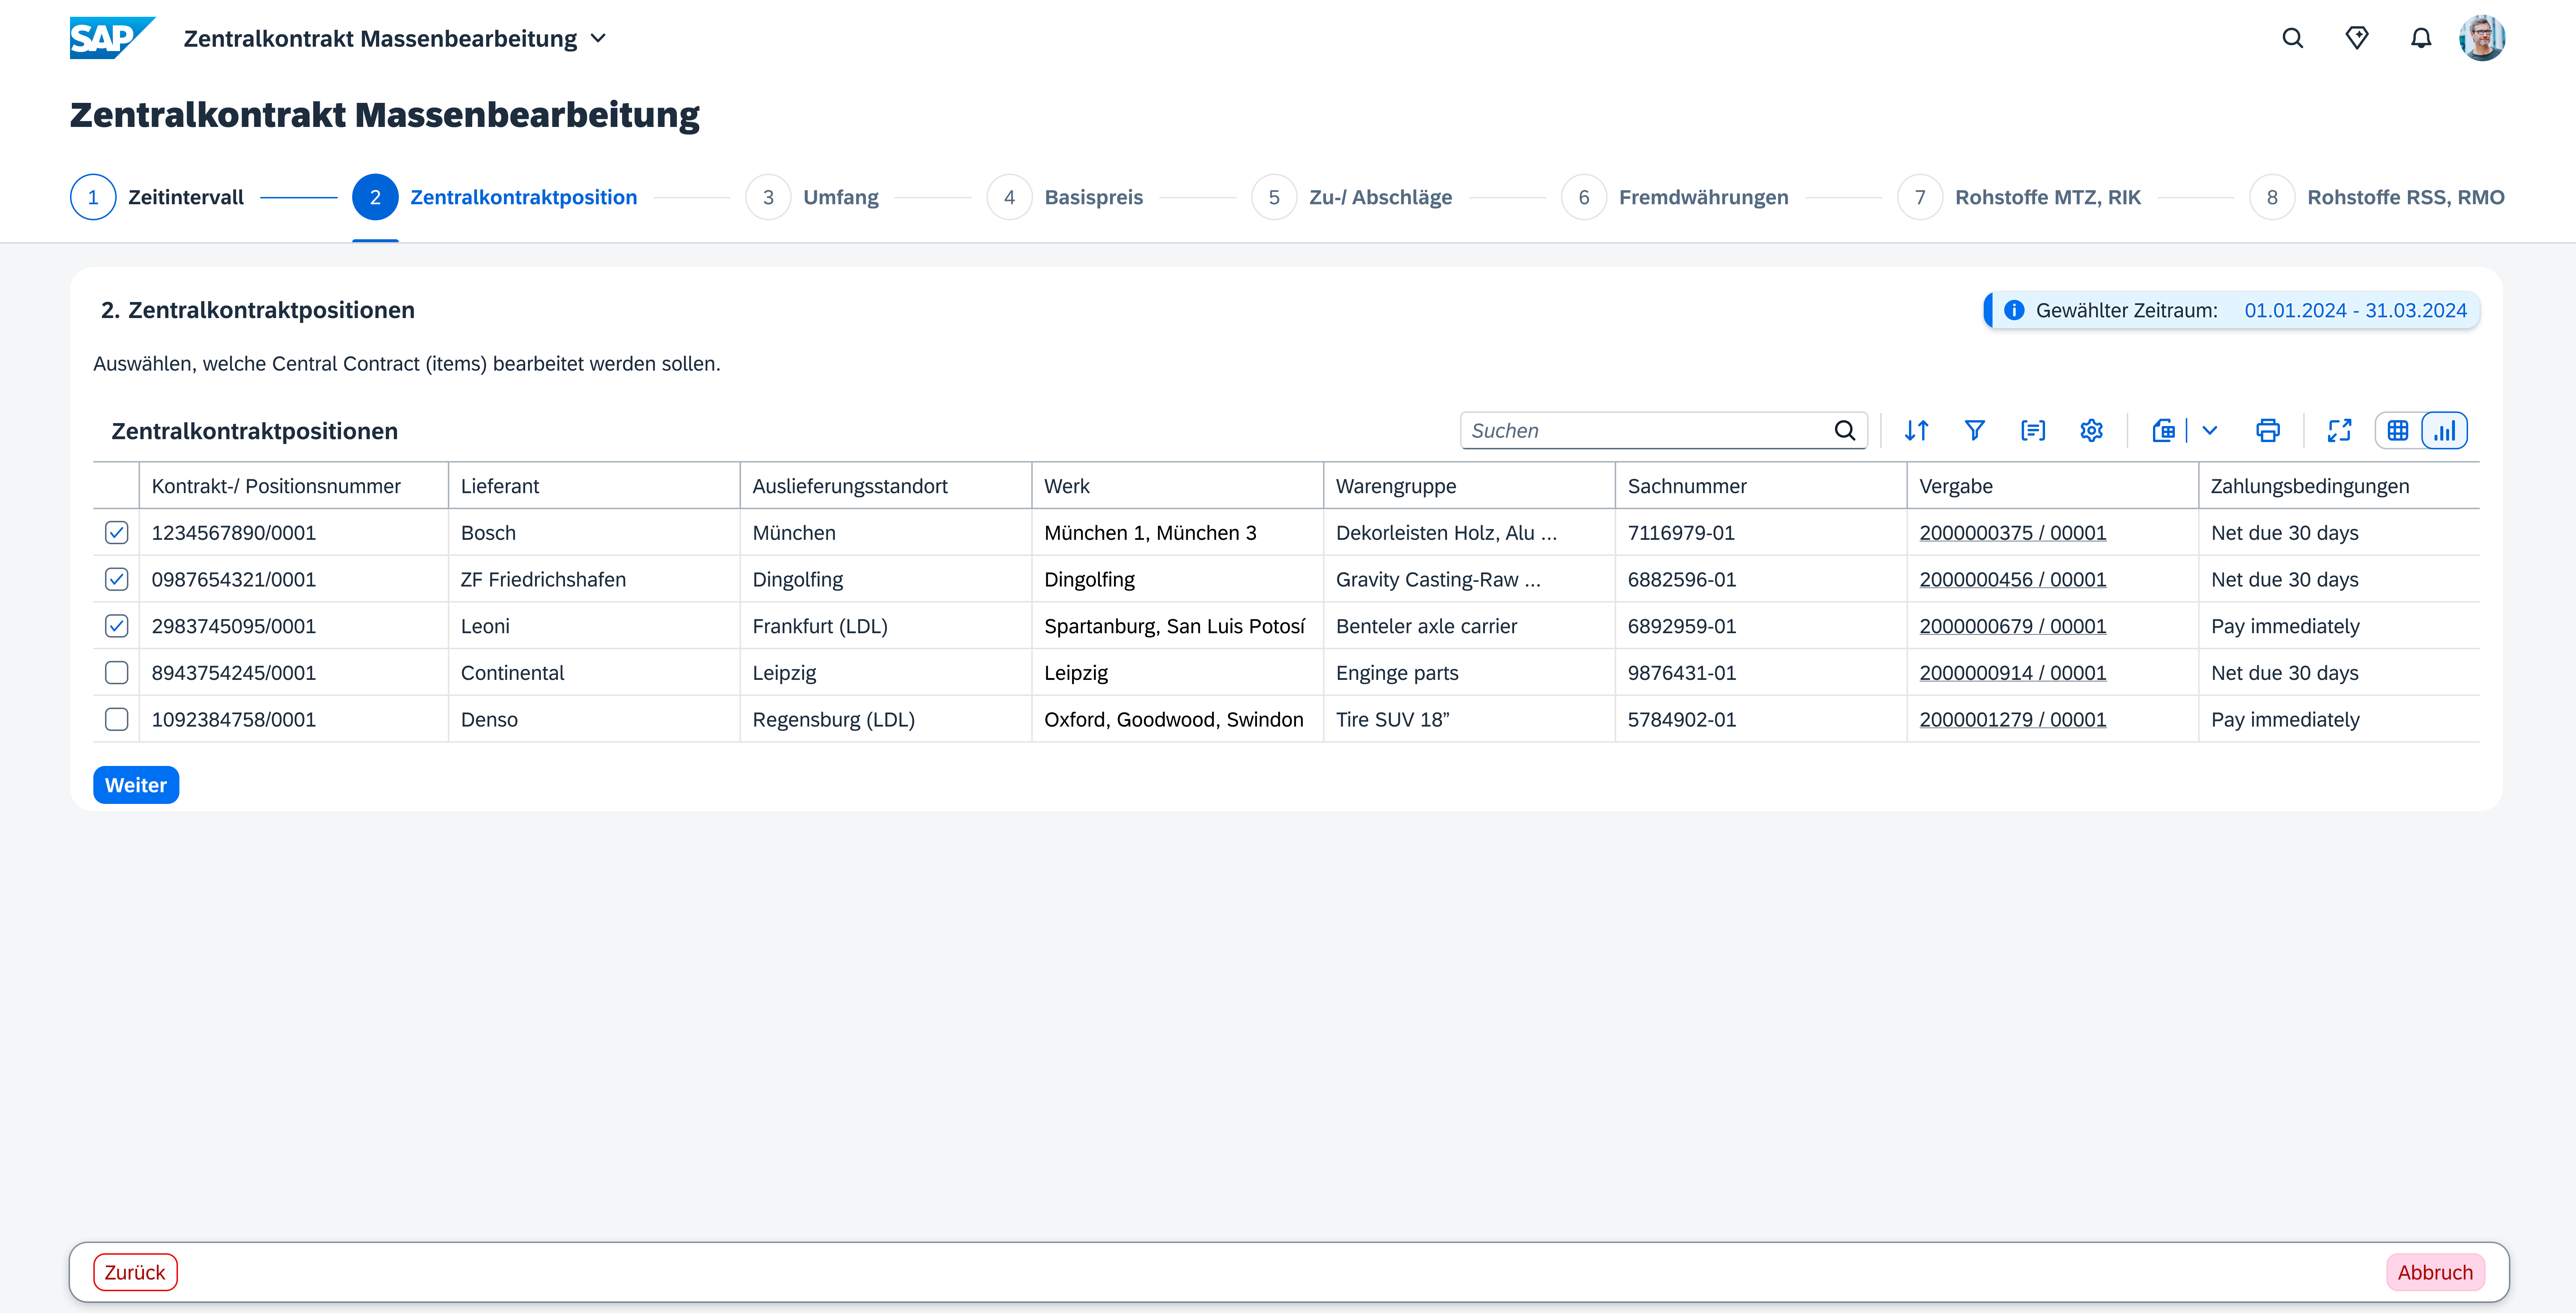
\includegraphics[height=7.66cm]{Bilder/Praxisteil-KL-Schritt-2.png}
    \caption[Kundenentwicklung, Massenbearbeitung Central Contracts, Auswahl der Zentralkontrakte]{Kundenentwicklung, Massenbearbeitung Central Contracts, Auswahl der Zentralkontrakte. Eigene Darstellung}
    \label{fig:PraxisKLSchritt2}
\end{figure}

Abbildung \ref{fig:PraxisKLSchritt2} zeigt den zweiten Schritt des Prozesses. Hier kann der Benutzer die Zentralkontrakte auswählen, die er bearbeiten möchte. Dazu stehen Filter-, Such- und Sortierfunktionen zur Verfügung. Des Weiteren kann die Tabelle exportiert und deren Darstellung verändert werden. Jedoch sind für den Facheinkäufer nur die Central Contracts sichtbar, die aufgrund der jeweiligen Rolle in dessen Verantwortungsbereich liegen. Durch Klicken auf die Checkboxen werden die Kontrakte selektiert. Zur Identifikation der zu ändernden Kontrakte wurden durch die Facheinkäufer wichtige Attribute identifiziert, die in der Tabelle abgebildet sind. Diese wird über eine Schnittstelle zum Zentralkontrakt befüllt. Auf einige Attribute soll nachfolgend genauer eingegangen werden. Die Kontrakt-/ Positionsnummer ist die eindeutige ID eines Zentralkontrakts. Deren letzter Teil ist immer 0001, da BMW immer für jede Position einen eigenen Kontrakt anlegt. Der Auslieferungsstandort kann sich von dem Werk, in dem die Teile verbaut werden, unterscheiden, wenn BMW ein Versorgungskonzept einsetzt.\footnote{Dies ist gekennzeichnet durch ''(LDL)'' (Logistik Dienstleister) hinter einem Wert in der Spalte Versorgungskonzept.} Letzteres ist eine Kostensparmaßnahme, da BMW die Bauteile vom Lieferanten an den nächstgelegenen Standort liefern lässt und von dort aus selbst logistisch an die Werke verteilt. Der Kunde gruppiert verschiedene Bauteile in Warengruppen, \zB Reifen oder Karosserie. Diese Bauteile werden im System durch Sachnummern abgebildet und identifizieren ein Bauteil, von der Entwicklung über seinen gesamten Lebenszyklus hinweg. Die Vergabe entspricht dem Sourcing Projekt aus dem ein Central Contract aus dem Product Sourcing System heraus erzeugt wird. 

\subsubsection{Auswahl des Umfangs der Massenbearbeitung}

\begin{figure}[H]
    \centering
    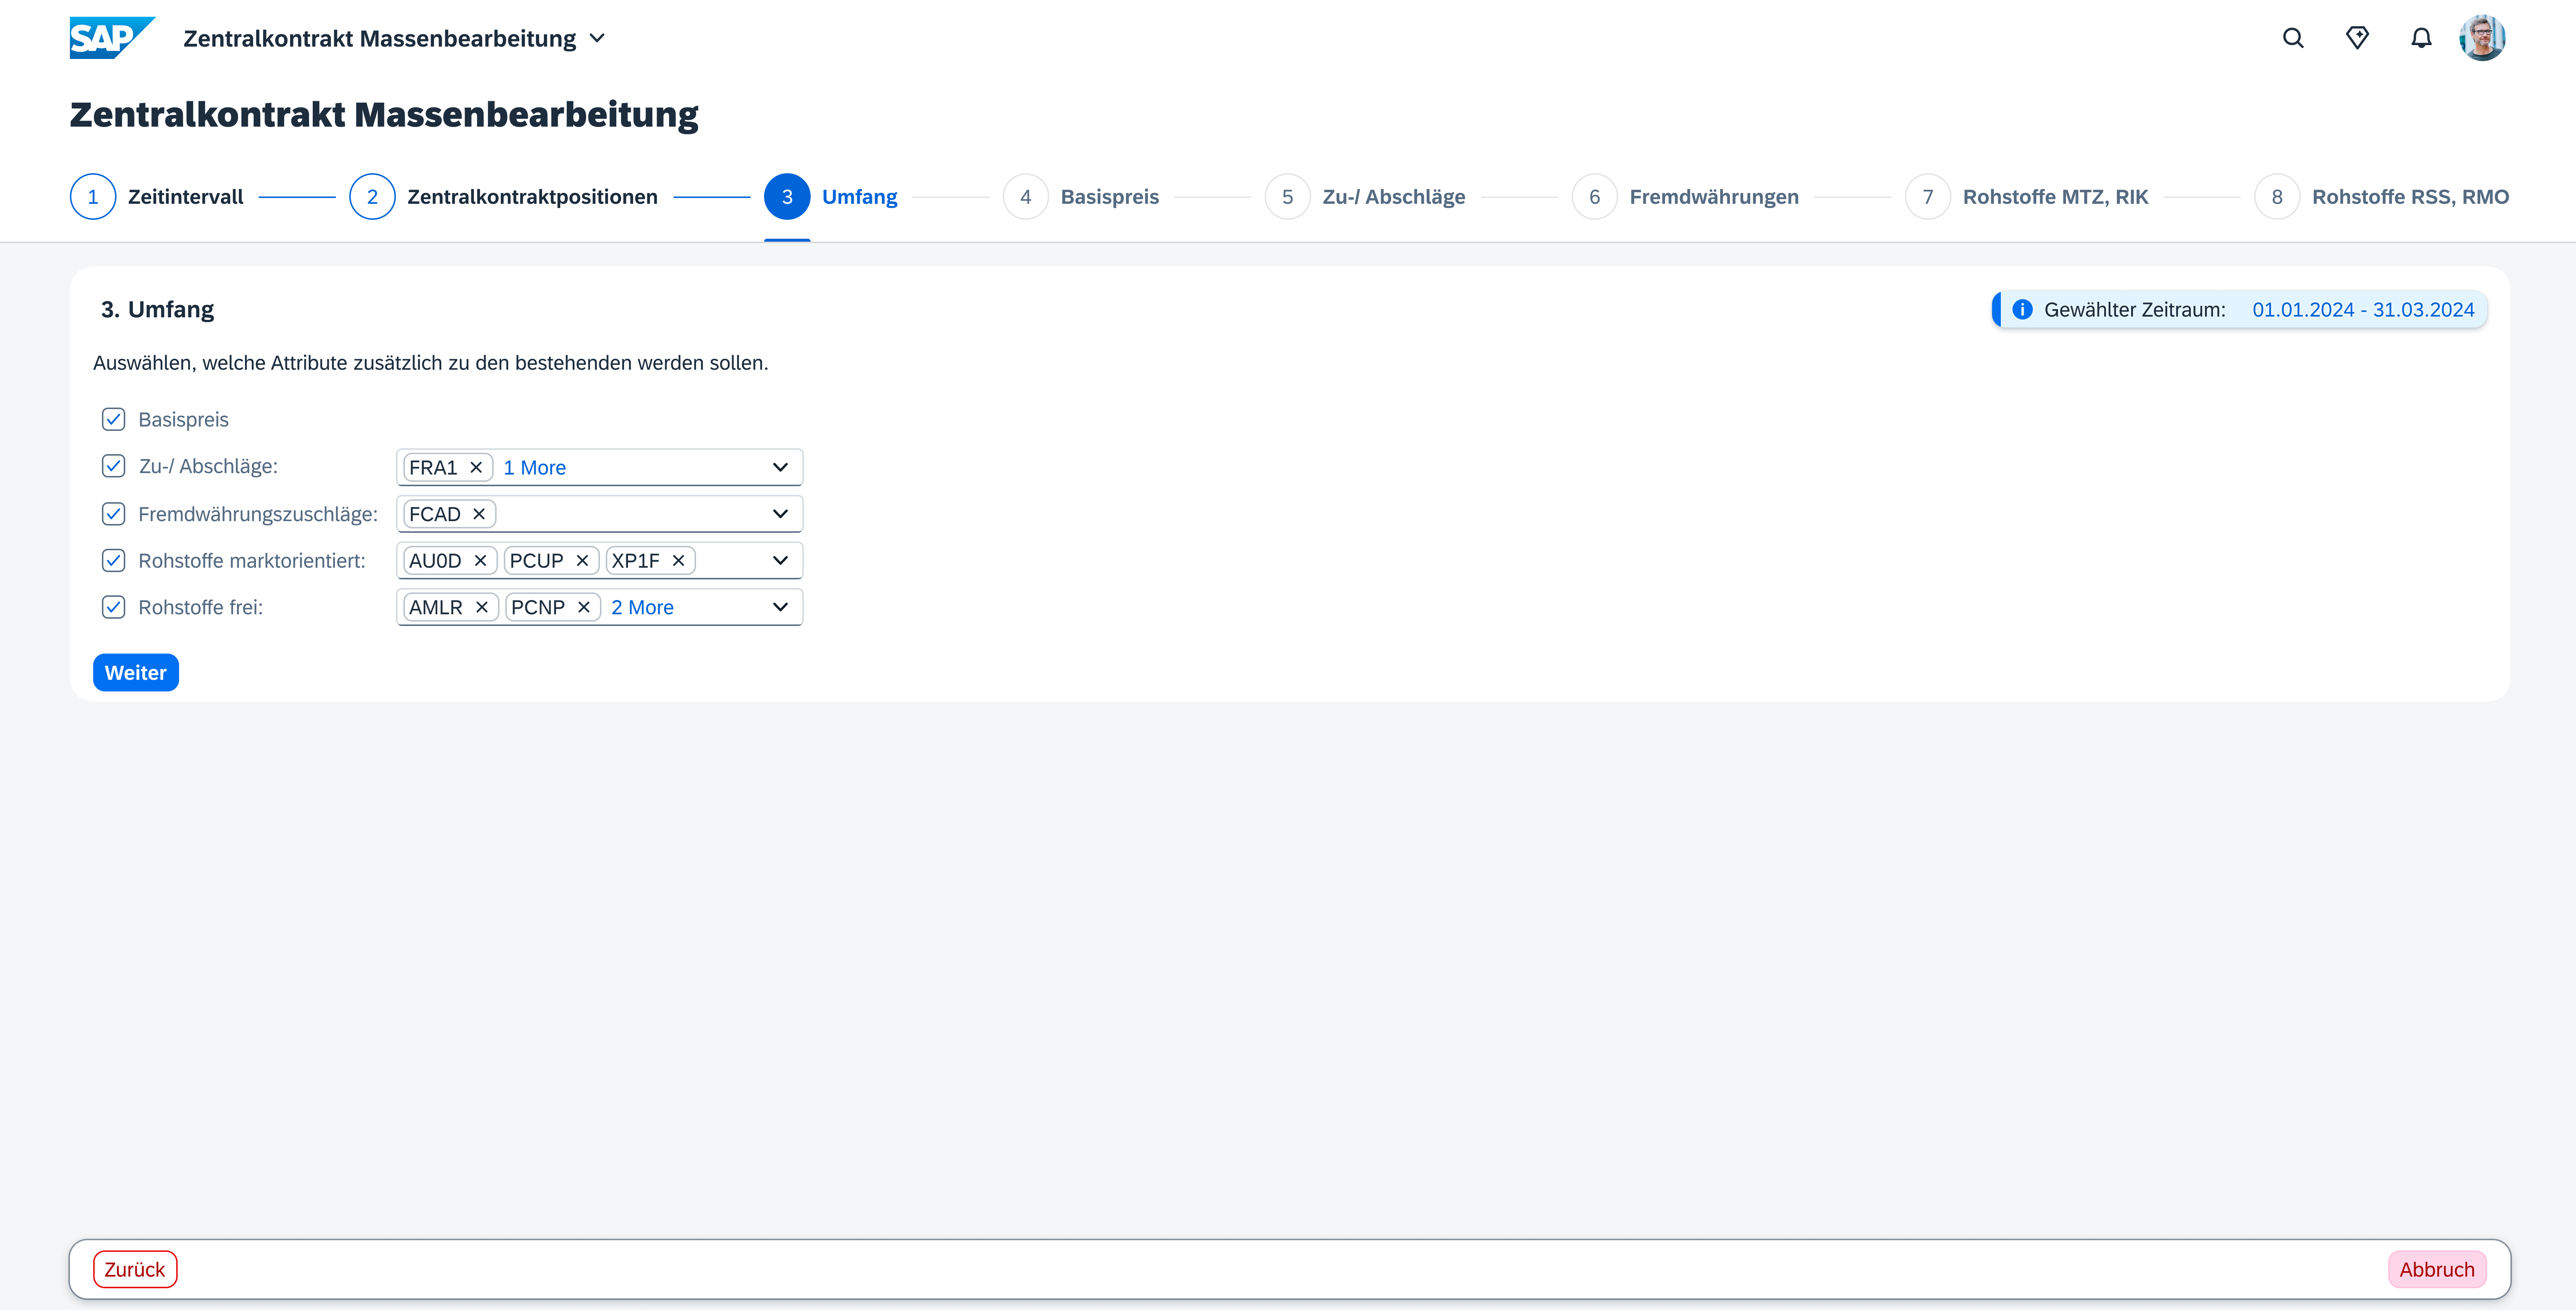
\includegraphics[height=7.65cm]{Bilder/Praxisteil-KL-Schritt-3.png}
    \caption[Kundenentwicklung, Massenbearbeitung Central Contracts, Auswahl der zu bearbeitenden Kategorien]{Kundenentwicklung, Massenbearbeitung Central Contracts, Auswahl der zu bearbeitenden Kategorien. Eigene Darstellung}
    \label{fig:PraxisKLSchritt3}
\end{figure}

Der letzte Schritt der Vorauswahl wird in Abbildung \ref{fig:PraxisKLSchritt3} dargestellt. Hier kann der Facheinkäufer durch Selektieren der Checkboxen auswählen, welche der fünf Kategorien der Zentralkontrakte er bearbeiten möchte. Sollte eine Kategorie nicht selektiert sein, wird der zugehörige Prozessschritt in der App ausgeblendet. In die Inputfelder neben den Kategorien kann der Endanwender einzelne Rohstoffe oder Konditionen, wie \zB Aluminium oder einen Verpackungszuschlag mittels deren ID eingeben. Durch diese Funktionalität können neue Konditionen oder Rohstoffe hinzugefügt werden, die in den Verträgen aktuell nicht vorhanden sind. Letztere werden den Tabellen im nächsten Schritt mit leeren Einträgen hinzugefügt. Alle im aktuellen Zeitintervall bestehenden Konditionen/ Rohstoffe werden, unabhängig von der Auswahl des Facheinkäufers ohnehin in den nächsten Schritten angezeigt. 

\subsubsection{Bearbeitung des Basispreises}

\begin{figure}[H]
    \centering
    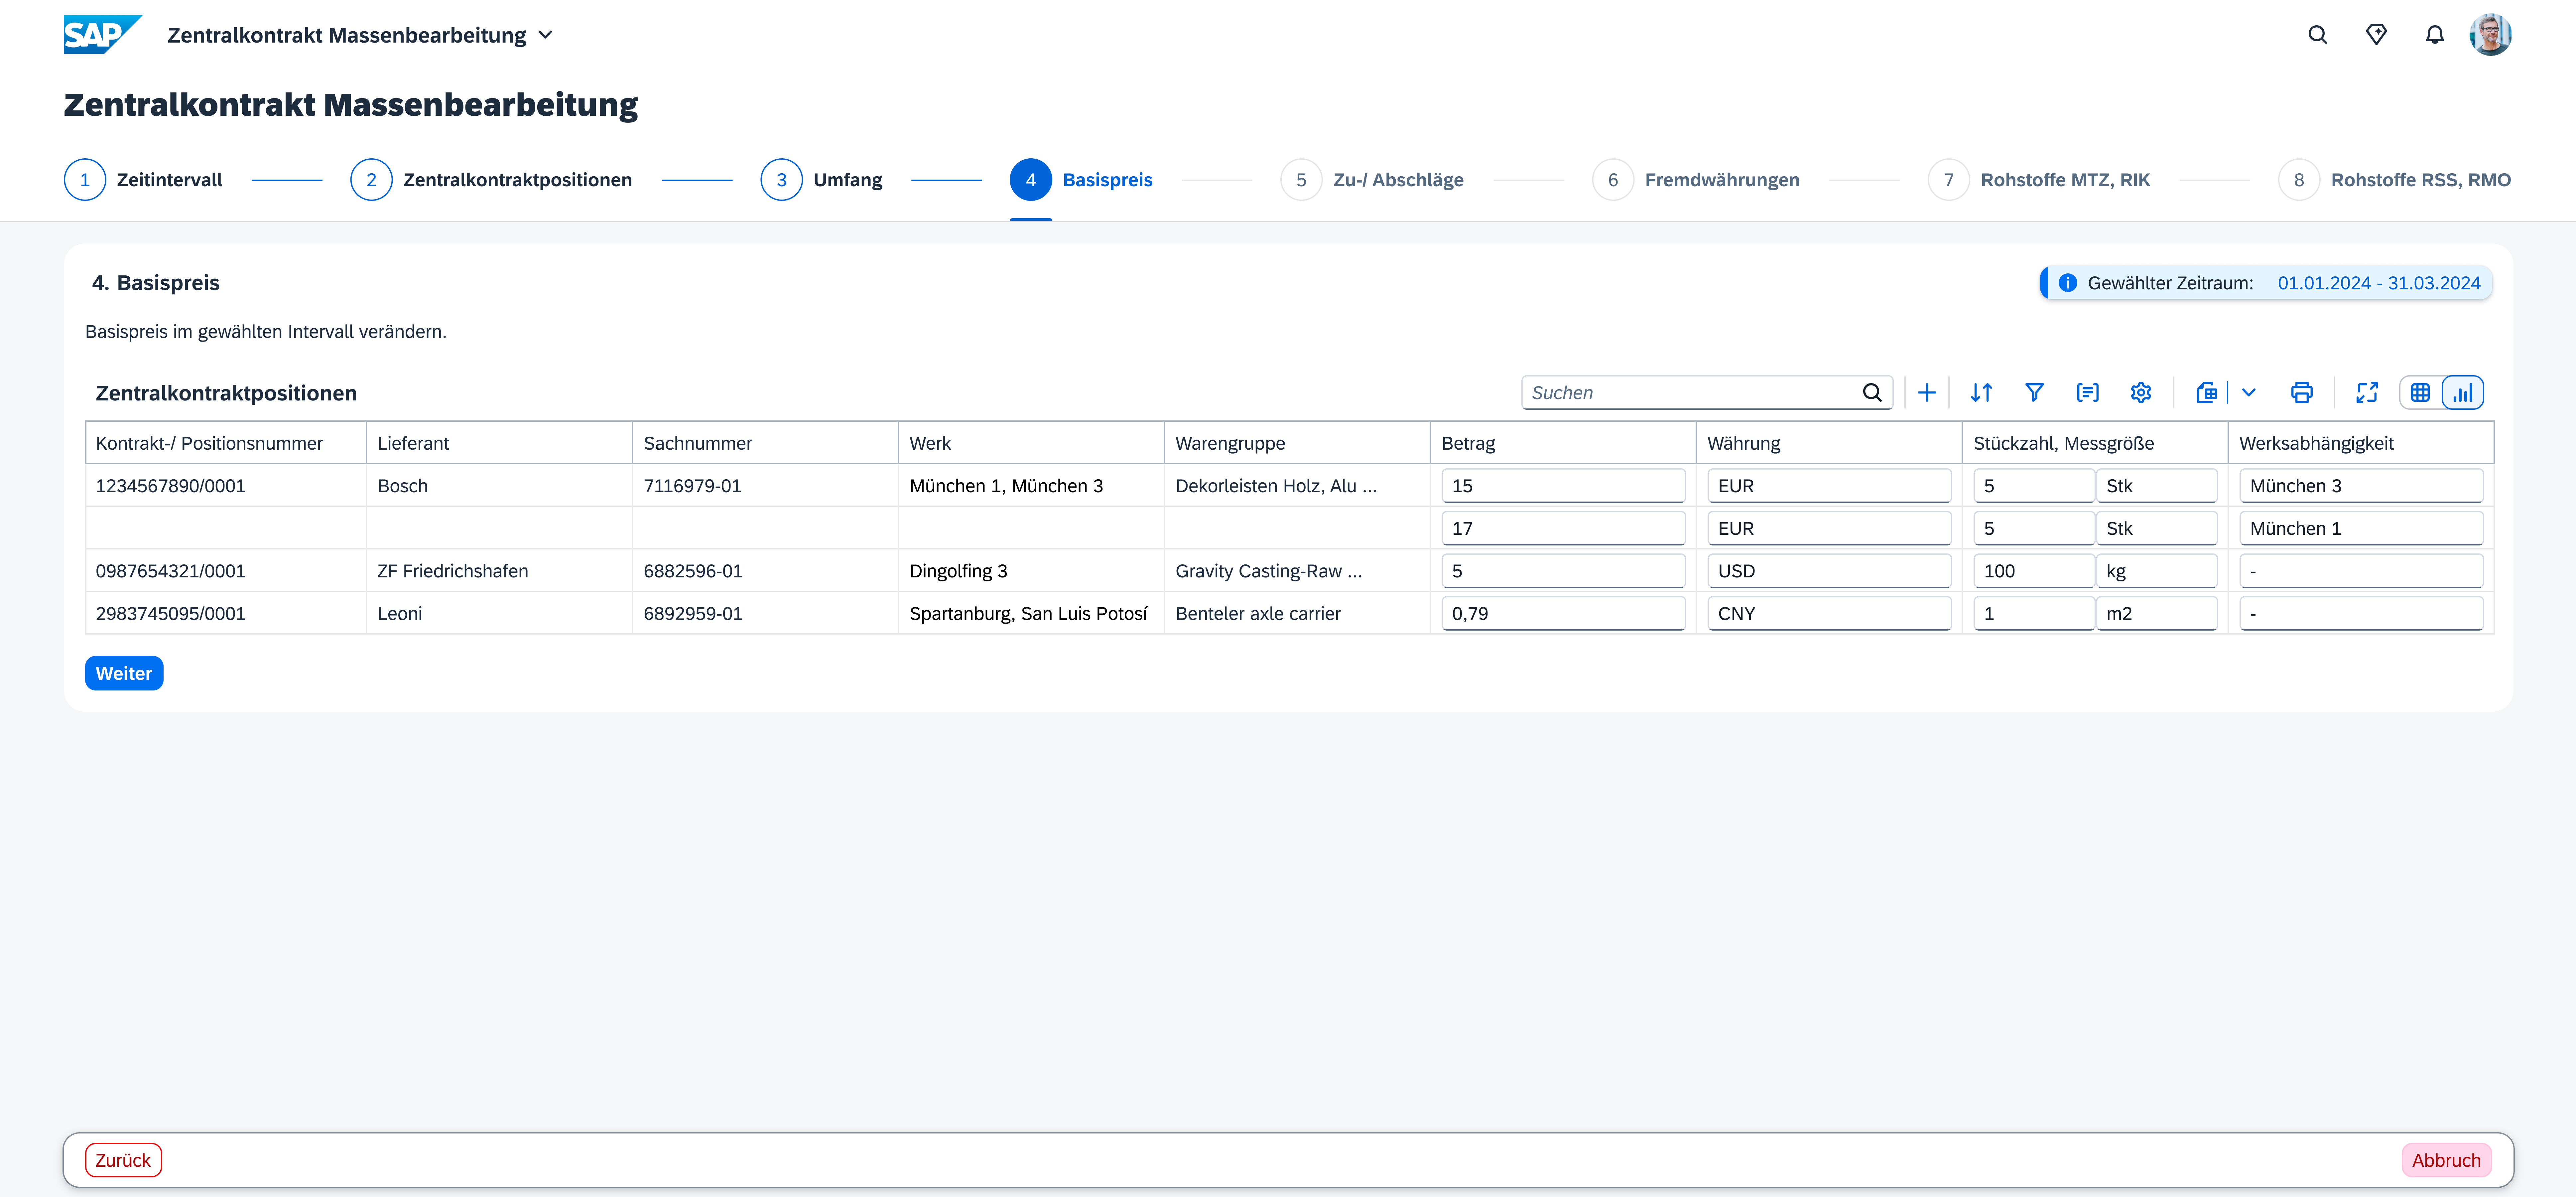
\includegraphics[height=6.99cm]{Bilder/Praxisteil-KL-Schritt-4.png}
    \caption[Kundenentwicklung, Massenbearbeitung Central Contracts, Bearbeitung des Basispreises]{Kundenentwicklung, Massenbearbeitung Central Contracts, Bearbeitung des Basispreises. Eigene Darstellung}
    \label{fig:PraxisKLSchritt4}
\end{figure}

In Abbildung \ref{fig:PraxisKLSchritt4} beginnt mit dem vierten Prozessschritt die Bearbeitungsphase mit dem Basispreis. Die Felder zur Identifikation der einzelnen Kontrakte wurden aus Übersichtlichkeitsgründen reduziert. Die jeweiligen Eingabefelder sind mit den im ausgewählten Zeitintervall gültigen Werten vorbefüllt. Sollten im gewählten Zeitintervall keine Werte vorhanden sein wären diese Felder leer. Wenn das gewählte Zeitintervall mehrere Instanzen des Basispreises mit verschiedenen Werten enthält, wird der Wert, der zu Beginn des gewählten Zeitraums gültig war, in das Feld eingetragen. Diese Logik gilt für alle weiteren anzupassenden Kategorien gleicherma\ss en. Sollte ein Vertrag werksabhängige Basispreise für verschiedene Lokationen haben, werden diese in der Tabelle in mehreren Zeilen untereinander aufgelistet. Zudem wird durch Eingaberegeln sichergestellt, dass entweder nur ein werksunabhängiger Basispreis existiert oder mehrere ausschlie\ss lich werksabhängige Basispreise. Die PME (Stückzahl, Messgrö\ss e) ist in zwei Eingabefelder aufgeteilt, um die Dateneingabe und -verarbeitung zu erleichtern. Falls ein Anwender die Dateneingabe in Excel präferiert, ist dies durch den Excel Up- und Download möglich. Es kann im Gegensatz zur Standardfunktionalität jedoch keine Datei für alle Kategorien heruntergeladen werden, sondern lediglich eine Datei pro Kategorie, die schematisch der in Abbildung \ref{fig:PraxisKLSchritt4} dargestellten Tabelle entspricht. Diese kann mit den aktuellen Werten befüllt heruntergeladen, angepasst und wieder hochgeladen werden. Somit kann die Fehlerbehandlung immer noch durch die App erfolgen, da eventuelle Falscheingabe farblich und mit einer Benachrichtigung hervorgehoben werden.

\subsubsection{Bearbeitung der Zu- und Abschläge}

\begin{figure}[H]
    \centering
    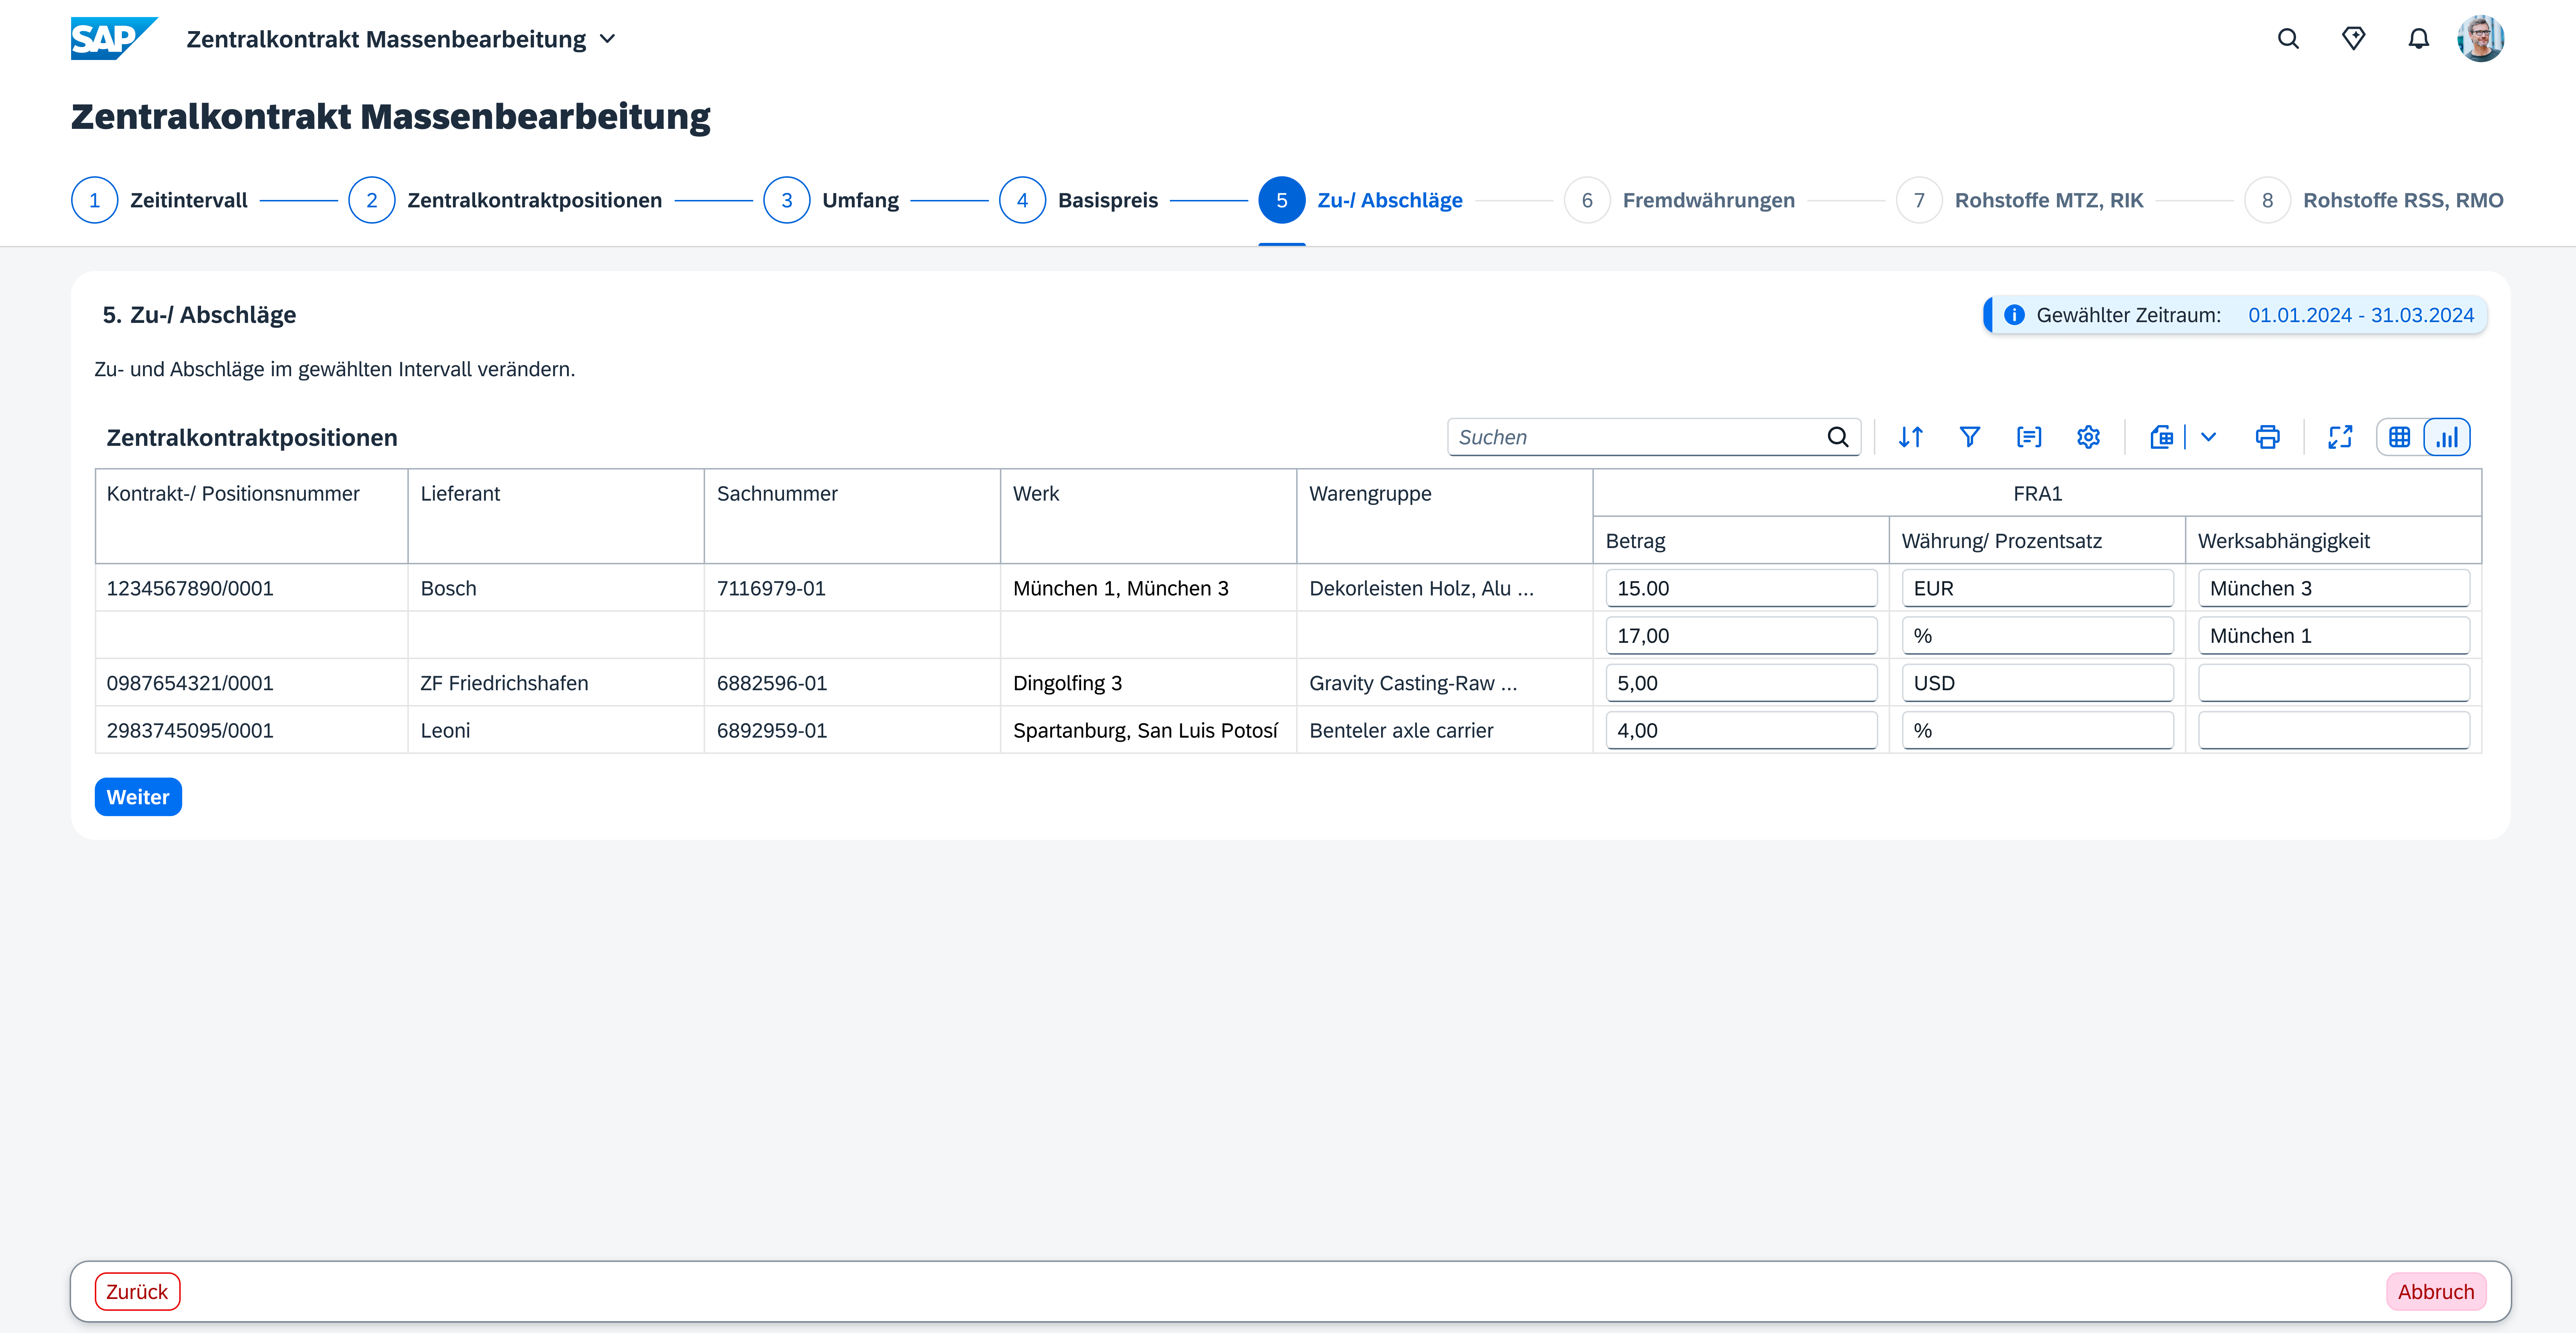
\includegraphics[height=7.78cm]{Bilder/Praxisteil-KL-Schritt-5.png}
    \caption[Kundenentwicklung, Massenbearbeitung Central Contracts, Bearbeitung der Zu- und Abschläge]{Kundenentwicklung, Massenbearbeitung Central Contracts, Bearbeitung der Zu- und Abschläge. Eigene Darstellung}
    \label{fig:PraxisKLSchritt5}
\end{figure}

Nachdem der Basispreis bearbeitet wurde, ist der nächste Schritt in Abbildung \ref{fig:PraxisKLSchritt5} die Bearbeitung der Zu- und Abschläge. Diese werden in der Tabelle in Spalten dargestellt, die sich in die je relevanten Felder unterteilen. Im konkreten Beispiel handelt es sich um einen Frachtzuschlag, der je nach Vertrag und Werksabhängigkeit andere Werte annehmen kann.\footnote{Aus Darstellungsgründen wurde auf die Darstellung mehrerer Zuschläge verzichtet. Diese würden analog zu ''FRA1'' rechts an die Tabelle ''angehängt'' werden. Selbiges gilt für die nächsten Kateogrien, die im Folgenden vorgestellt werden.} In allen editierbaren Kategorien - au\ss er des Basispreises - können \zB einzelne Rohstoffe oder Zu-/ Abschläge für einen Kontrakt gelöscht werden. Dies wird durch das Löschen aller Werte in den entsprechenden Feldern eines Zuschlags für einen bestimmten Vertrag durchgeführt. Der Basispreis hingegen kann für ein gültiges Zeitintervall nicht gelöscht, sondern nur überschrieben werden, da sonst Lücken im Preisverlauf entstehen würden. 

\subsubsection{Bearbeitung der Fremdwährungen}

\begin{figure}[H]
    \centering
    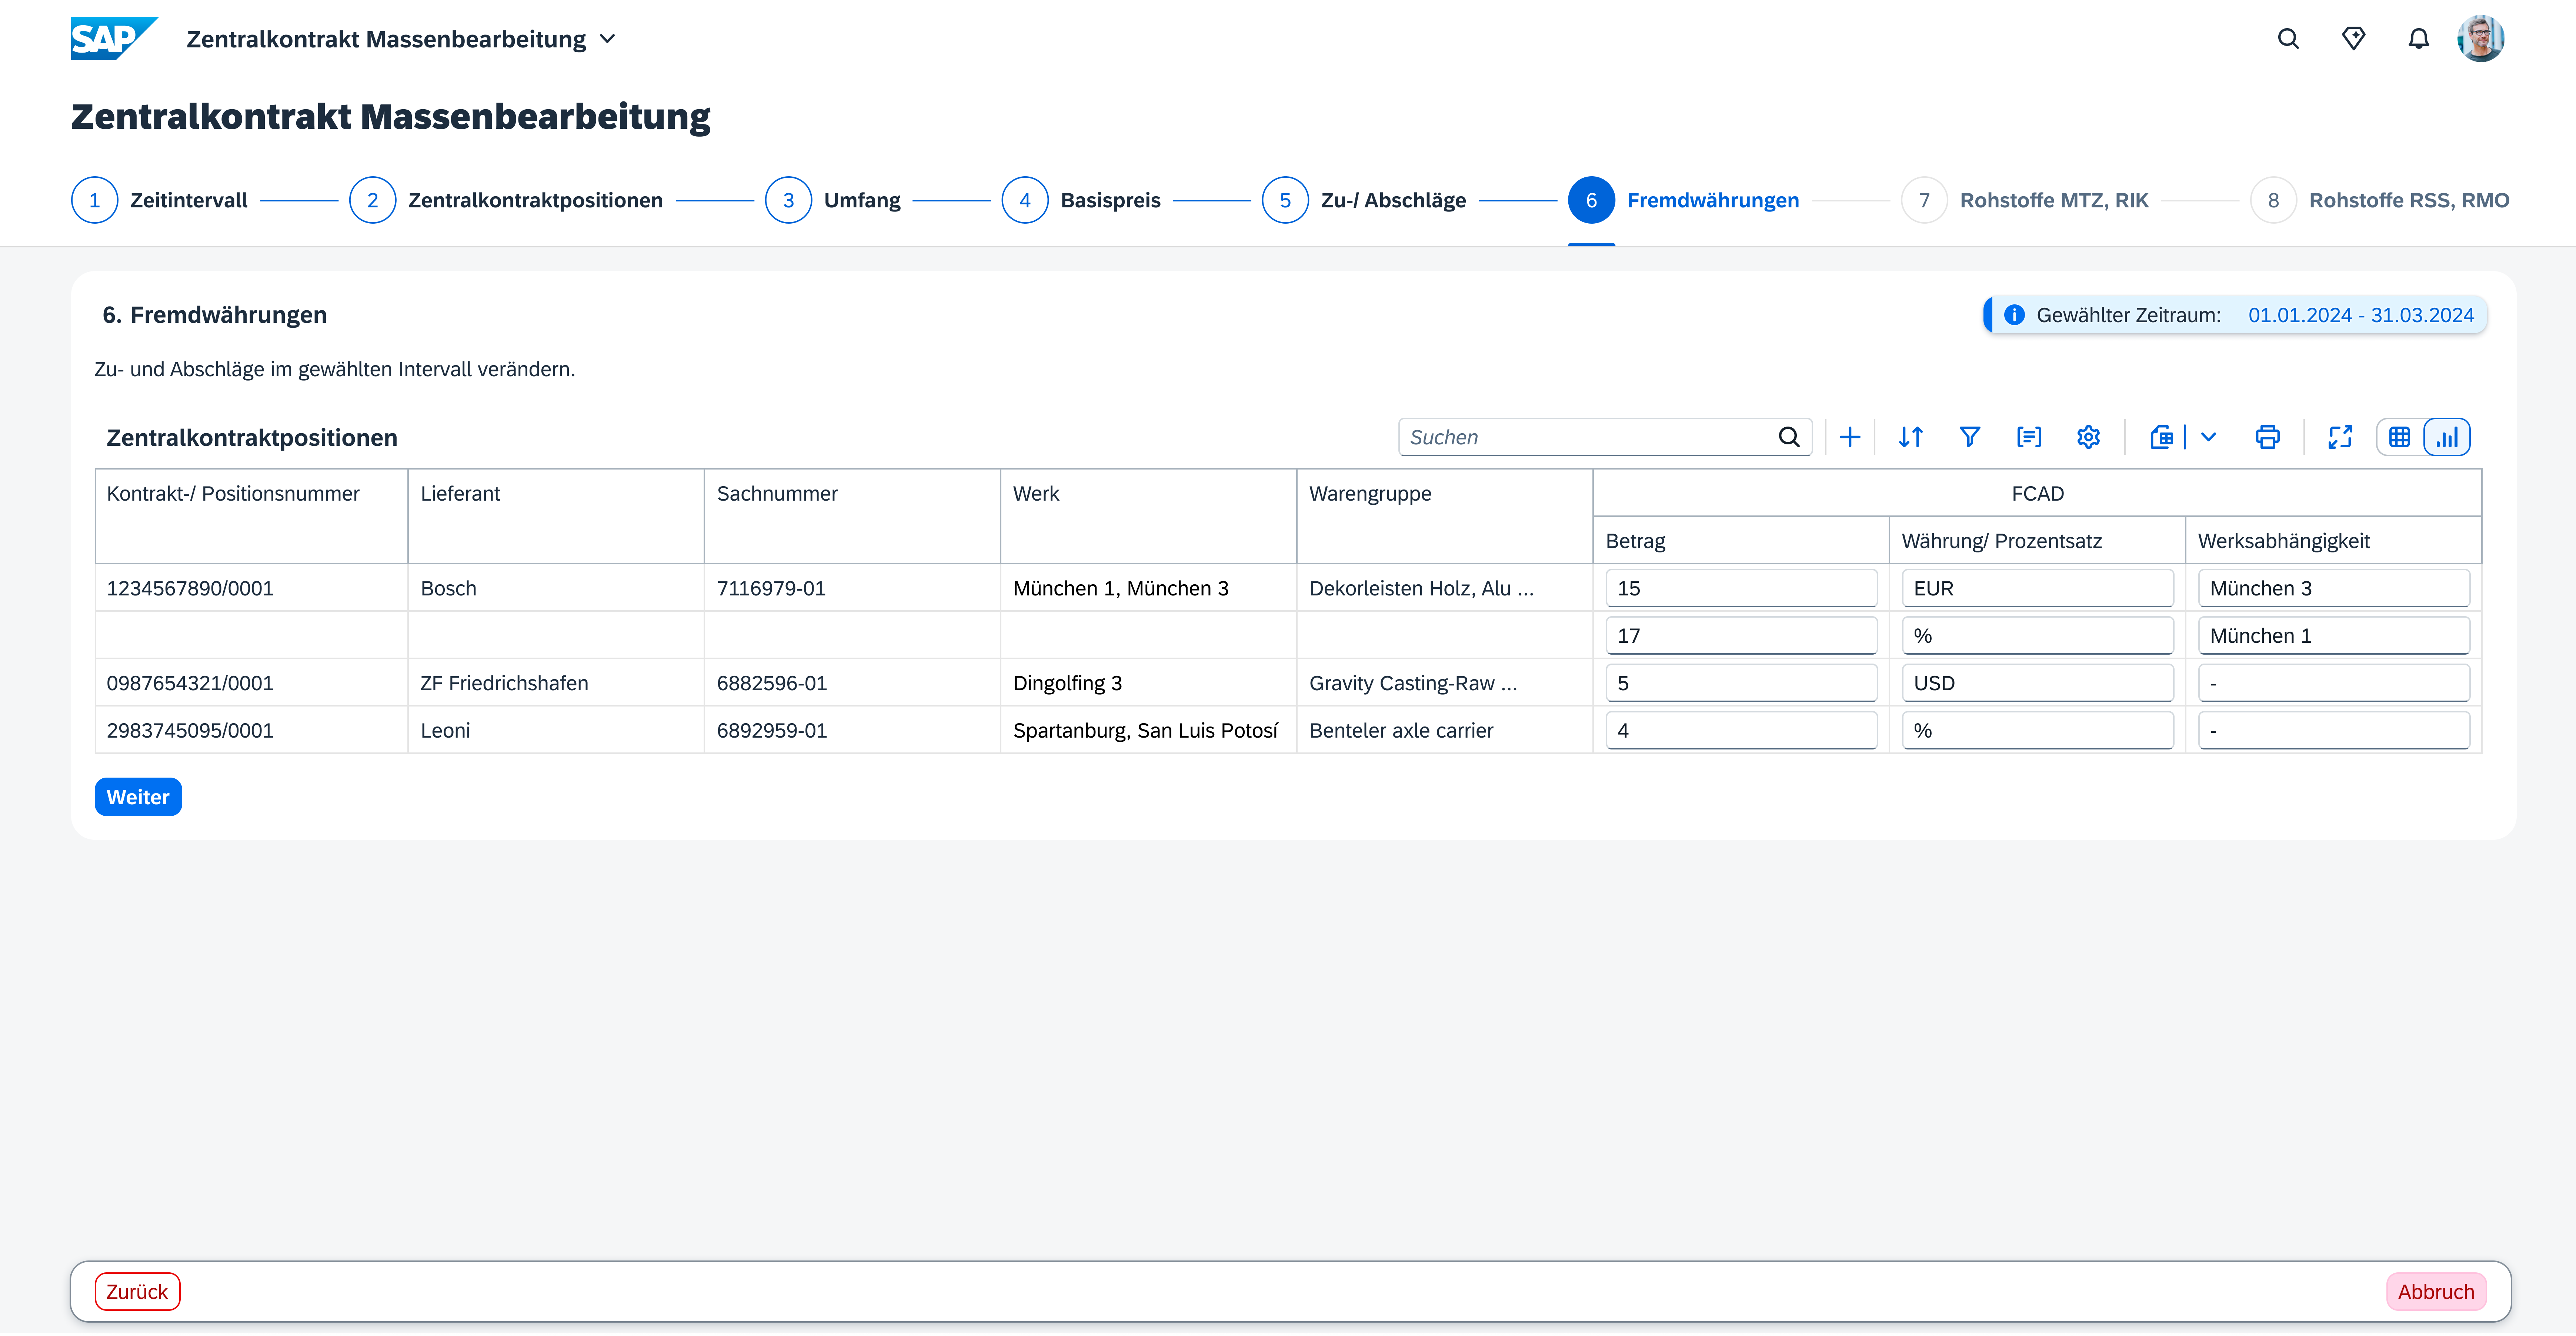
\includegraphics[height=7.78cm]{Bilder/Praxisteil-KL-Schritt-6.png}
    \caption[Kundenentwicklung, Massenbearbeitung Central Contracts, Bearbeitung der Fremdwährungen]{Kundenentwicklung, Massenbearbeitung Central Contracts, Bearbeitung der Fremdwährungen. Eigene Darstellung}
    \label{fig:PraxisKLSchritt6}
\end{figure}

Die nächste Konditionsart sind Fremdwährungen, die in Abbildung \ref{fig:PraxisKLSchritt6} dargestellt sind. Diese sind im Bezug auf die benötigten Felder analog zu den Zu- und Abschlägen aufgebaut. Die Trennung von Zu-/ Abschläge und Fremdwährungen in zwei Kategorien ist durch den Arbeitsablauf der Facheinkäufer bedingt. Der Unterschied besteht lediglich darin, dass der Zweck spezialisiert ist, um internationale Währungsdifferenzen zu berücksichtigen. Beispielsweise könnte BMW im Kontext des dritten Vertrags einen Fremdwährungszuschlag verhandeln, um internationale Transaktionskosten zu kompensieren.

\subsubsection{Bearbeitung der marktorientierten Rohstoffe}

\begin{figure}[H]
    \centering
    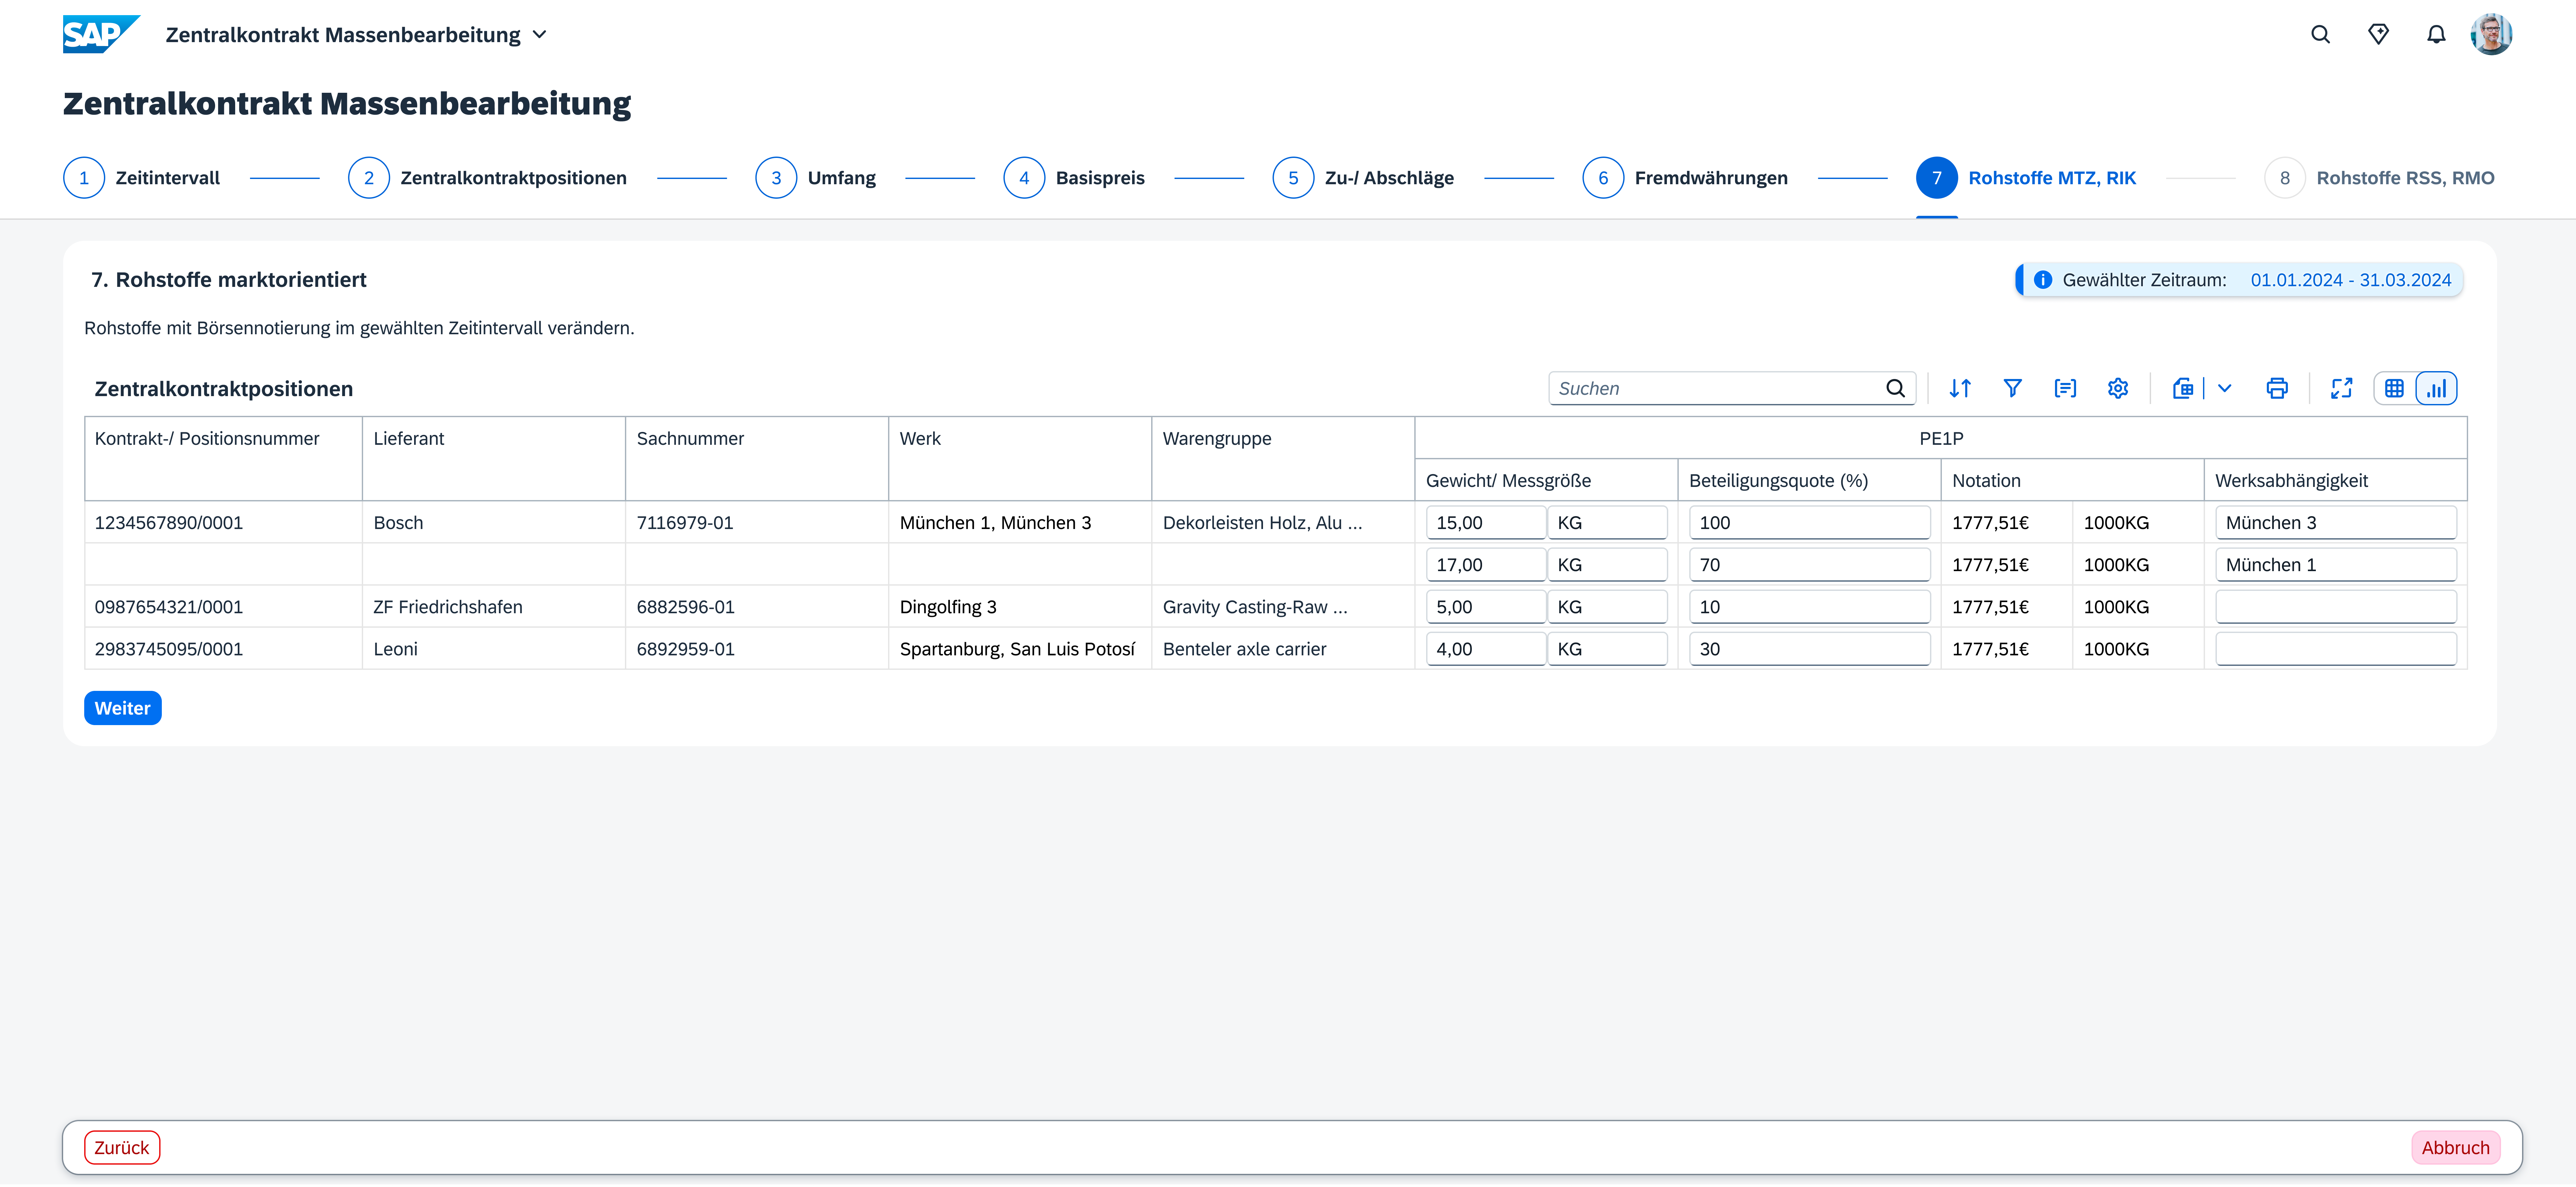
\includegraphics[height=6.91cm]{Bilder/Praxisteil-KL-Schritt-7.png}
    \caption[Kundenentwicklung, Massenbearbeitung Central Contracts, Bearbeitung der marktorientierten Rohstoffe]{Kundenentwicklung, Massenbearbeitung Central Contracts, Bearbeitung der marktorientierten Rohstoffe. Eigene Darstellung}
    \label{fig:PraxisKLSchritt7}
\end{figure}

Die letzten beiden Kategorien, die der Endanwender bearbeiten kann, sind Rohstoffe. In Abbildung \ref{fig:PraxisKLSchritt7} ist die Maske für marktorientierte Rohstoffe dargestellt. Da die Notationen der RMO vom organisierten Markt vorgegeben werden, sind diese als normale Textfelder angelegt und somit nicht durch den Anwender veränderbar. Letztere ist zudem in zwei Felder aufgegliedert, da der Preis sich immer auf eine bestimmte Menge des Rohstoffs bezieht. Um die gesamte preisliche Auswirkung auf den Basispreis zu erfassen, ist zudem noch die Menge des Rohstoffs, die für ein Bauteil benötigt wird, zu erfassen. Abhängig von der Art des Bauteils kann diese Menge in verschiedenen Einheiten angegeben werden. Beispielsweise wäre in einem Karosseriebauteil wesentlich mehr Aluminium enthalten, als in einem Computerchip Silizium enthalten ist. Die eingegebenen Daten werden noch mit der Beteiligungsquote multipliziert, um den tatsächlichen Rohstoffpreis in einem Bauteil zu berechnen.

\subsubsection{Bearbeitung der Rohstoffe mit freier Notierung}

\begin{figure}[H]
    \centering
    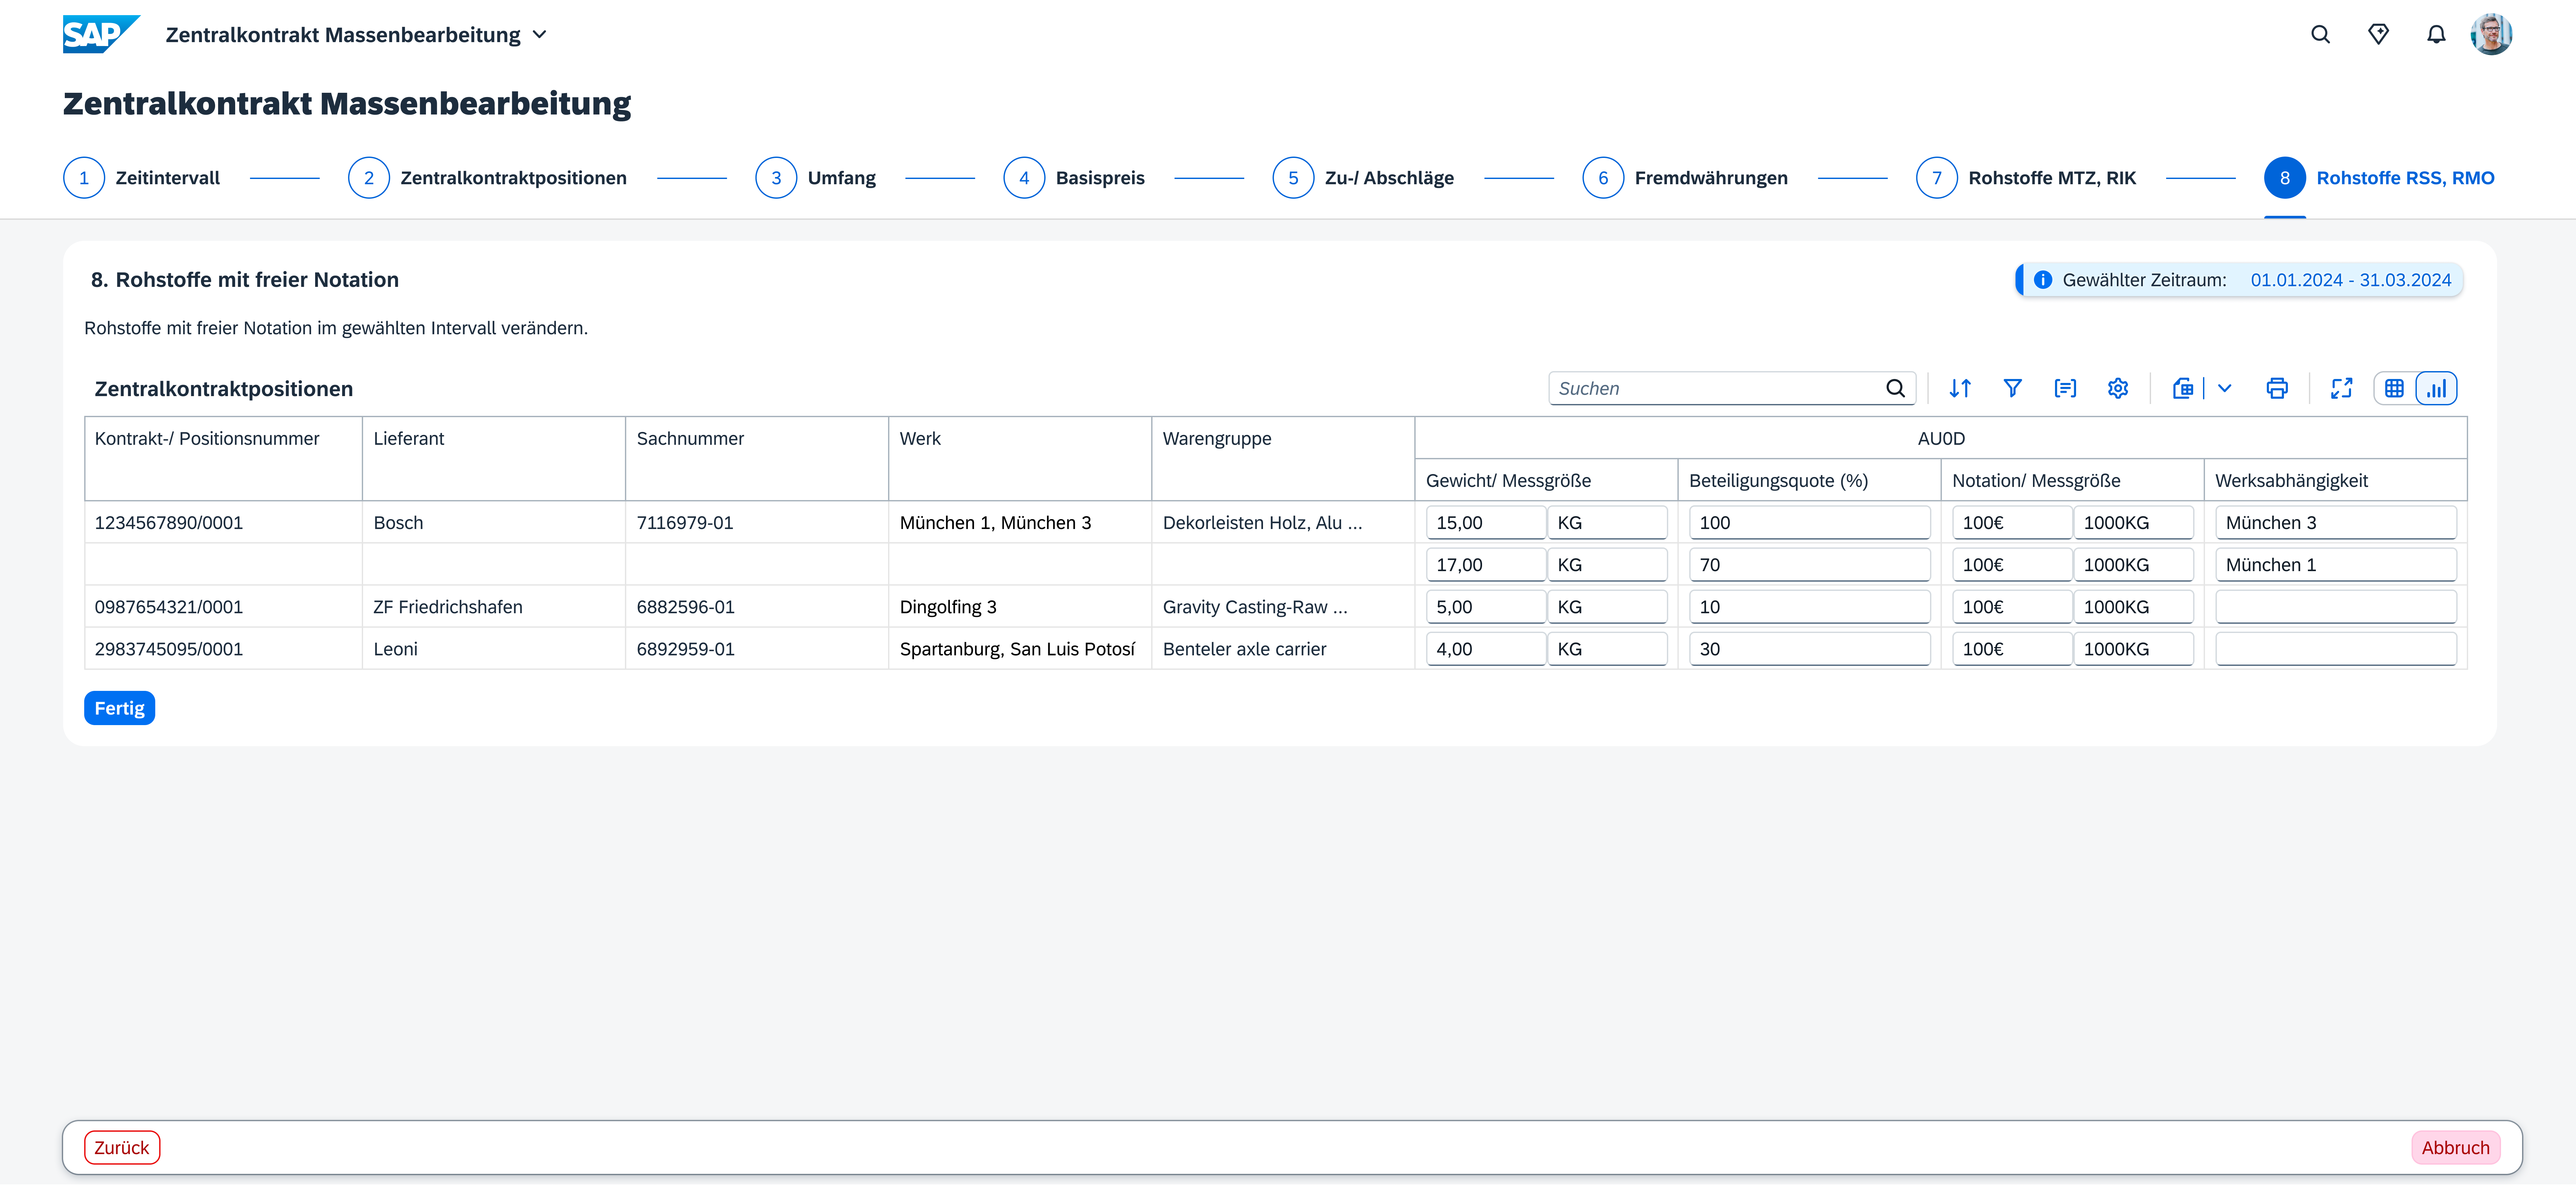
\includegraphics[height=6.91cm]{Bilder/Praxisteil-KL-Schritt-8.png}
    \caption[Kundenentwicklung, Massenbearbeitung Central Contracts, Bearbeitung der Rohstoffe mit freier Notierung]{Kundenentwicklung, Massenbearbeitung Central Contracts, Bearbeitung der Rohstoffe mit freier Notierung. Eigene Darstellung}
    \label{fig:PraxisKLSchritt8}
\end{figure}

Der letzte Prozessschritt ist die Bearbeitung der Rohstoffe mit freier Notierung. Diese sind in Abbildung \ref{fig:PraxisKLSchritt8} dargestellt und ebenfalls ähnlich zu den RMO aufgebaut. Der Unterschied besteht darin, dass die Preise nicht vorgegeben werden, sondern vom Facheinkäufer selbst gepflegt werden können. Aus diesem Grund ist die Notation als Inputfeld angelegt.

Nachdem der Einkäufer alle Änderungen bestätigt hat, wird im Hintergrund die Schnittstelle ''MM\_PUR\_UPDATE\_CCTR\_FROM\_RENEGO'' der Lösung Contract Price Renegotiation aufgerufen. Diese übernimmt einerseits die Anpassung der Preisgültigkeiten (automatische Verkürzung und Verlängerung der Basispreis-Intervalle, quartalsweise Trennung von Rohstoffgültigkeiten) und andererseits die Übernahme der Daten ins System. Mit diesem Schritt ist der Prozess abgeschlossen.

\section{Evaluation der verschiedenen Lösungsansätze}

Nachdem beide Lösungsansätze vorgestellt wurden, sollen diese nun mittels einer Nutzwertanalyse evaluiert und gegeneinander abgewogen werden. Im Folgenden werden beide Varianten anhand der Kriterien Entwicklungs- und Schulungsaufwand, Wartungsaufwand, funktionaler Erfüllungsgrad der Anforderungen, Zeit zur Implementierung, Migrations- und Integrationsmöglichkeiten, Anpassbarkeit und User Experience bewertet. Die Bewertungsskala reicht von eins (sehr schlecht) bis fünf (sehr gut). Aus den Bewertungen wird dann eine Gesamtpunktzahl ermittelt, um eine Handlungsempfehlung für den Kunden abzugeben.

\subsubsection{Kosten}

Unter den Kosten sind die gesamten initialen Kosten zu verstehen, bis die Lösung erstmalig im produktiven Einsatz ist, sowie die laufenden Kosten für die Betreuung des Systems nach diesem Zeitraum. Diese Kosten setzen sich zum einen aus dem Entwicklungsaufwand zusammen. Hier fallen Kosten, wie beispielsweise für die Entwicklung der App selbst, die Einrichtung dieser, sowie die Integration an bestehende Systeme an. Zum anderen fallen Kosten für die Schulung des Personals an, um mit der neuen Lösung arbeiten zu können. Geschult werden müssen unter anderem die Administratoren, die die nach Ende des Projekts für den Betrieb der Software verantwortlich sind, sowie die Supportmitarbeiter, die den Endanwendern bei Problemen mit der Lösung helfen, als auch die Facheinkäufer, die diese in ihrem beruflichen Alltag nutzen müssen. Die Wartungskosten setzen sich aus der Behebung von Fehlern oder Anpassungen der Software, den laufenden Endanwendersupport und allgemeinen Wartungskosten, wie Updates, etc. zusammen.

Hier ist die Standardlösung mit drei von fünf Punkten als neutral zu bewerten. Vor allem der Entwicklungsaufwand ist hier gering, da es sich um eine SAP-Standard-Funktionalität handelt, die lediglich im Rahmen des Customizings angepasst werden muss. Da neben dem normalen Customizing im Bezug auf die Excel-Tabelle zusätzlich ein BAdI implementiert werden muss, um die kundenspezifischen Anforderungen im Bezug auf zeitliche Gültigkeiten einzelner Preisbestandteile, Prüfungen und Berechtigungen umzusetzen, entstehen hier dennoch nicht unerhebliche Aufwände. Der Schulungsaufwand ist hier für Administratoren und den Support moderat, da sich die Software bis auf den BAdI im Rahmen des SAP-Standard bewegt und für diesen Schulungen angeboten werden. Zudem wird aufgrund weniger Fehlerquellen eine nicht so umfassende Expertise benötigt. Für die Facheinkäufer ist der Schulungsaufwand eher hoch, da die Lösung nicht dem definiertem Prozess entspricht und somit eine höhere Fehleranfälligkeit besteht. Die Wartung der Standardlösung verursacht eher niedrige Kosten, da die App an sich von SAP gewartet wird und somit Fehlerbehebungen und allgemeine Wartungskosten, abgesehen von der BAdI-Implementierung nicht anfallen. Hier entstehen lediglich Aufwände für den funktionalen Support der Einkäufer.

Die kundenspezifische Lösung erhält hingegen einen von fünf Punkten. Diese unzureichende Wertung lässt sich durch die au\ss erordentlich hohen Entwicklungsaufwände erklären. Die App muss, abgesehen von der Fiori-Benutzeroberfläche von Grund auf neu entwickelt werden. Dies beinhaltet die Systemarchitektur, die Implementierung der Geschäftslogik und die Anbindung an andere Systeme. Aus diesem Grund ist auch der Schulungsaufwand für Administratoren und den Support sehr hoch, da diese sich tief in die Software einarbeiten müssen. Zudem gibt es keine offiziellen Schulungen oder Dokumentationen. Für den Endanwender ist der Schulungsaufwand geringer, da die Lösung genau auf dessen Bedürfnisse zugeschnitten ist und somit eine geringere Fehleranfälligkeit besteht. Die Wartungsaufwände der kundenspezifischen Lösung sind ebenfalls sehr hoch, da diese allein in der Verantwortlichkeit des Kunden liegt. Somit fallen Kosten für die Behebung von Fehlern, Anpassungen der Software, den laufenden Endanwendersupport und allgemeinen Wartungskosten an.

\subsubsection{Funktionalität}

Das Kriterium der Funktionalität beschreibt den Grad, zu dem die funktionalen Anforderungen durch eine Lösung erfüllt werden. Diese Anforderungen untergliedern sich jeweils in die neu definierte Prozessstruktur und die Anforderungen an das Systemverhalten.

Die Standardlösung erhält in dieser Kategorie zwei von fünf Punkten, da die Anforderungen an das Systemverhalten zwar umgesetzt werden können, jedoch die Prozessstruktur nicht dem definierten Prozess entspricht. Dies ist vor allem auf die fehlende Möglichkeit, die Massenänderung durch eine Vorauswahl der Rahmenbedingungen Zeitintervall, Verträge und Umfang der Änderung einzugrenzen. Dies hat zur Folge, dass die Excel bei der Bearbeitung von vielen Verträgen mit vielen Konditionen/ Rohstoffen sehr unübersichtlich wird, wenn der Facheinkäufer gleichzeitig noch die verschiedenen zeitlichen Gültigkeiten der einzelnen Preisbestandteile und deren Abhängigkeiten untereinander berücksichtigen muss. In diesem Fall kommt die Lösung dem Status quo sehr nahe, der, aufgrund der unzulänglichen UX und hohen Fehlerquote, der initiale Grund für die Optimierung im Rahmen dieser Arbeit ist. Somit kann dieser Ansatz nicht als geeignet angesehen werden. Es werden dennoch zwei Punkte vergeben, da die Anforderungen an das Systemverhalten umgesetzt werden können.

Die kundenspezifische Lösung erzielt in dieser Kategorie fünf von fünf Punkten, da sowohl die Prozessstruktur, als auch die Anforderungen an das Systemverhalten vollständig umgesetzt werden. Die App ist so konzipiert, dass der Facheinkäufer seine Aufgaben in seinem natürlichen Arbeitsfluss erledigen kann, während er durch die Fehlerbehandlung und Validierung des Systems unterstützt wird. 

\subsubsection{Implementierungszeit}

Die Implementierungszeit ist der Zeitraum bis die Lösung erstmalig im produktiven Einsatz ist. Hierbei sind sowohl die Entwicklungszeit, als auch die Zeit für die Schulung des Personals zu berücksichtigen. Aufgrund der Interdependenzen der verschiedenen IT-Systeme und der Beteiligung verschiedener Abteilungen mit begrenzten zeitlichen Kapazitäten, kann dieses Kriterium zudem nicht beliebig über Einsatz finanzieller Ressourcen gesteuert werden.

Die Standardlösung erreicht in dieser Kategorie vier von fünf Punkten, da die Implementierungszeit ist hier relativ kurz, da die Fiori-App Teil des Standards ist und das Customizing in der SAP-Umgebung eher geringe Aufwände verursacht. Die Implementierung der BMW-spezifischen Geschäftslogik ist jedoch zeitintensiv. Für die Schulung administrativer und operativer Benutzer zusätzlich Zeit eingeplant werden.

Die kundenspezifische Lösung erhält beim Kriterium Implementierungszeit analog zu den Kosten einen von fünf Bewertungseinheiten. Die Zeitspanne bis die App produktiv eingesetzt werden kann ist bei dieser Variante sehr lang, da die gesamte App entwickelt werden muss und lediglich auf eine Schnittstelle zum Zentralkontrakt zurückgegriffen werden kann. Zudem können die Schulungszeiten für Administratoren und Supportmitarbeiter als zeitintensiv eingestuft werden, da diese sich fundamental in die Software einarbeiten müssen. Für die Facheinkäufer ist der Schulungszeitraum hingegen kürzer, da die Software deren Anforderungen exakt erfüllt. 

\subsubsection{Migrations- und Integrationsmöglichkeiten}

Migrations- und Integrationsmöglichkeiten sollen einerseits darstellen, wie gut die Lösung in die bestehende Systemlandschaft integriert werden kann. Andererseits ist ein wichtiges Kriterium, ob ein Umstieg von der entwickelten Lösung zurück auf den SAP-Standard möglich wäre. Dies ist relevant, da seitens der SAP Verbesserungen der aktuellen Massenbearbeitungsfunktionalität für BMW in Aussicht gestellt wurden und es in einem solchen Fall aufgrund der Weiterentwicklung und Wartung durch SAP nicht durch BMW getragen werden müsste.

Die Standardlösung erhält in dieser Kategorie vier von fünf Punkten, da die Lösung als SAP-Entwicklung sehr gut in die bestehende Systemlandschaft integriert werden kann und hier diverse Schnittstellen zur Verfügung stehen. Da die Fiori-App bereits Teil der Standardfunktionalitäten ist, ist das zweite Kriterium ohnehin gegeben.

Mit drei von fünf Bewertungseinheiten ist die BMW-spezifische Lösung als etwas schlechter einzustufen. Die Integration in die bestehende Systemlandschaft ist aufgrund der flexiblen Architektur der App ebenso wie bei der Variante des Standards gegeben. Die Migrationsmöglichkeiten der Massenbearbeitung in den Standard gestaltet sich jedoch schwieriger, da die App speziell auf BMW zugeschnitten und die Wahrscheinlichkeit, dass die App in dieser Form auch von anderen Kunden benötigt wird, eher niedrig ist. Zudem würde eine Migration erhebliche Aufwände für die Endanwender darstellen.

\subsubsection{Anpassbarkeit}

Unter der Anpassbarkeit ist zu verstehen, wie gut die Lösungen an zukünftige Anforderungen angepasst werden können. Hierbei ist zu berücksichtigen, dass in Zukunft gegebenenfalls weitere Bereiche des Zentralkontrakts massenhaft gepflegt werden müssen, oder dass sich die Preislogiken \zB aufgrund regulatorischer Änderungen anpassen müssen.

Aufgrund der eingeschränkten Anpassbarkeit wird der Ansatz im Rahmen des Standards zu bleiben mit zwei Punkten bewertet. Dies ist grö\ss tenteils darauf zurückzuführen, dass die Fiori-App an sich nicht angepasst werden kann und somit auch bei weiteren zukünftigen Anwendungsbereichen Probleme entstehen könnten. Nichtsdestotrotz kann im Bezug auf das Systemverhalten durch die Implementierung von BAdIs eine gewisse Anpassbarkeit erreicht werden.

Dem entgegen steht die Eigenentwicklung für BMW mit fünf von fünf Bewertungseinheiten. Die App ist so konzipiert, dass sie flexibel an zukünftige Anforderungen angepasst werden kann. Sollten sich die Anforderungen an die Massenbearbeitung ändern, können diese durch Anpassungen in der Software umgesetzt werden, da die Entwicklungsmöglichkeiten uneingeschränkt sind. 

\subsubsection{User Experience}

Unter dem Kriterium User Experience werden im Folgenden die Aspekte Nützlichkeit und Bedienbarkeit zusammengefasst, um zu bewerten, wie gut die Lösung von den Endanwendern angenommen wird. 

Die der Ansatz des angepassten Standards erzielt in dieser Kategorie ebenfalls zwei von fünf Punkten. Die Nützlichkeit der Lösung selbst ist gegeben, da alle Preisbestandteile des Zentralkontrakts bearbeitet werden können und die Anforderungen an das Systemverhalten erfüllt werden können. Dennoch ist die Bedienbarkeit der Standard-App als unzulänglich zu bewerten, da durch die fehlende Vorauswahl zu viele Informationen zu vieler Dimensionen in einem Arbeitsblatt vorhanden sind. Das führt zu einer hohen Fehleranfälligkeit und hohen nachgelagerten Aufwänden für die Systemadministratoren. Zudem ist infrage zu stellen, ob die Lösung von den Endanwendern akzeptiert wird, da die Handhabung der Software schlecht ist.

Im Gegensatz zur Fiori-App des Standards können für die kundenspezifische Eigenentwicklung fünf von fünf Bewertungseinheiten vergeben werden. Die Nützlichkeit der Lösung ist gegeben, da alle Preisbestandteile des Zentralkontrakts bearbeitet werden können und die Anforderungen an das Systemverhalten erfüllt werden können. Die Bedienbarkeit der App ist als sehr gut zu bewerten, da die Software exakt auf die Anforderungen der Facheinkäufer zugeschnitten ist und somit eine geringe Fehleranfälligkeit besteht. Zudem ist davon auszugehen, dass die Lösung von den Endanwendern akzeptiert wird, da die Handhabung der Software intuitiv ist.

\subsubsection{Gesamtbewertung}

Über alle sechs Kriterien können beide Lösungen maximal 30 Punkte erreichen. Die Standardlösung erzielt in Summer 17 Punkte und der Ansatz der Eigenentwicklung 20 Punkte. Somit erreicht letztere drei Punkte mehr und somit ein ca. 17,6\% besseres Ergebnis als die der Ansatz des Standards. Damit ist die Eigenentwicklung der Alternative vorzuziehen.